%% ----------------------------------------------------------------
%% Thesis.tex
%% ---------------------------------------------------------------- 
\documentclass[oneside]{ecsthesis}      % Use the Thesis Style

\graphicspath{{../Figures/}}   % Location of your graphics files
\usepackage{natbib}            % Use Natbib style for the refs.
\hypersetup{colorlinks=true}   % Set to false for black/white printing
\input{Definitions}            % Include your abbreviations
\usepackage{booktabs}
\usepackage{graphics}
\usepackage{graphicx}
\usepackage{float}
\usepackage{rotating}
\usepackage{longtable} % for 'longtable' environment
\usepackage{pdflscape} % for 'landscape' environment
\usepackage{array} % for extrarowheight
\usepackage{latexsym}

%% ----------------------------------------------------------------
\begin{document}
\frontmatter
\title      {A Web Application Using Open Data and Data Visualisation for Higher Education Destination Choices in The UK}
\authors    {\texorpdfstring
             {\href{mailto:sw9n14@ecs.soton.ac.uk}{SHANCHUAN WU (sw9n14)
}}
             {SHANCHUAN WU}
            }
            
     
%\supervisor {Dr. Mark J Weal}
\addresses  {\groupname\\\deptname\\\univname}
\date       {\today}
\subject    {}
\keywords   {}

\maketitle

\begin{abstract}
With the contemporary globalisation, the number of international students in the UK has risen strongly over the last decade. When international students choose universities and cities for their higher education, they will take many different factors into consideration. Therefore, international students’ higher education destination choice involves multiple factors. Some of these factors play a vital role in this decision-making process. There are many potential benefits of open data for higher education, and one of them is to help students make informed education decisions.  Data visualisation is a powerful tool to represent and analyse the data, so it becomes essential for decision making. 

This dissertation identified some significant factors that influence the decision-making process of international students in the UK for their higher education and implemented a web application to visualise open data about these factors. This web-based application proved to be helpful for international students when they decide destination cities and universities for their higher education in the UK.

\end{abstract}
\tableofcontents
\listoffigures
\listoftables
%\lstlistoflistings
%\listofsymbols{ll}{$w$ & The weight vector}
\acknowledgements{I would like to express my deepest appreciation to my supervisor, Dr. Mark J Weal, for the continuous support of my dissertation and project, for his patience, motivation, and immense knowledge. His guidance helped me in all the time of project and writing of this dissertation.

Besides, I would like to thank my examiner, Dr. Elena Simperl, for her valuable advice and suggestions for my project and dissertation.

My sincerely thank also goes to my friends and classmates in University of Southampton. In particular, I am grateful to two of my best friends, Chunhui Zhou and Chaofeng Zhou, for enlightening me on system development.


Last but not the least, I would like to thank my family: my parents and brother for supporting me spiritually throughout writing this dissertation and my life in general.}
%\dedicatory{To \dots}
\mainmatter
%% ----------------------------------------------------------------
%% ----------------------------------------------------------------
%% Introduction.tex
%% ---------------------------------------------------------------- 

\chapter{Introduction} \label{Chapter:Introduction}
In recent years, there has been a tremendous growth in the number of international students who choose to study abroad for their higher education \cite{ahmad2015investigation}. The decision-making process for higher education destination choices is a highly complicated process that is subject to multiple factors. Understanding how international students’ decision-making process regarding higher education destination choices can help them make informed decisions. Open data is widely used in various areas, and it proves to have great benefits in higher education. On the other hand, well-designed data graphics or charts are usually the simplest and the most powerful way to help the users think visually \cite{aljehane2015visualizing}, so data visualisation is also applied in higher education to allow international students to gain information on destination cities or universities straightforwardly and interactively. Therefore, it is a great value to combine data visualisation with open data to help international students make informed decisions for their higher education destination choices.



\section{Problem Statement
}

The impacts of economic and social events are likely to change the factors in the international students’ decision-making process for higher education. Some determining factors may become less important, while some less important factors may attract international students’ more attention. The result of Brexit Poll, for instance, is possible to motivate international students to focus on the location of destination universities or cities, because universities or cities near London can provide them with more opportunities to get work permits after graduation. Hence, it is necessary to conduct a survey to identify current determining factors that influence international students’ decision-making process to help them choose destination universities or cities in the UK. There are millions of open datasets in the world, so it is necessary to search for or collect relevant open datasets that reflect those factors influencing higher education destination choices. Moreover, with the advancement of visualisation techniques, it is also important to choose suitable techniques to visualise these open datasets to help students make informed decisions.



\section{Aims and Objectives 
}

The major aim of the project is to develop a web-based application that uses data visualisation techniques to visualise open data to help international students’ make informed decisions for their higher education destination universities or cities. The project also aims to research international students’ decision-making process for higher education and identify current significant factors in this process. The functionality and the user interface of the system will be aligned with those factors.

To accomplish the specified aims of this project, the objectives defined below identify the process that will be followed throughout the project.
\begin{itemize}


	\item Analyse and summarise current key factors that influence international students’ higher education destination choices in the UK.
 
	\item Search for or collect relevant open data that can present those significant factors affecting higher education destination choices.
  
	\item Investigate and identify advanced visualisation techniques that are suitable for visualising the important factors. 

	\item Apply appreciate data visualisation techniques in designing a web application that includes all significant factors and provides international students with comprehensive descriptions of destination universities or cities in the UK.

	\item Test and evaluate the web application to identify whether this application is helpful for international students to make informed decisions for their destination universities or cities.
\end{itemize}

\section{Dissertation Structure
}
The following chapters will emphasise on the procedures of analysing and developing a web-based application to visualise open data in higher education throughout the phases of this project. Specifically, the background research conducted related to the factors influencing higher education destination choices and the application of open data and data visualisation in educational choices is presented in chapter 2. Chapter 3 will introduce information on project management, such as project constraints, project methodology, time management as well as risk analysis and management. Subsequently, chapter 4 and chapter 5 will cover system analysis and system design respectively. Afterwards, chapter 6 will recount the implementation outcomes of this system based on system analysis and design in last two chapters, and introduce the highlighted features implemented in this system; Furthermore, the methodologies and procedures for testing and evaluation will be described in chapter 7. Eventually, the conclusion, critical reflection and future work will be given in chapter 8.


%% ----------------------------------------------------------------
%% Background.tex
%% ---------------------------------------------------------------- 

\chapter{Background Research} \label{Chapter:Background Research}

This chapter will summarize the background research of this project, which focuses on the factors influencing international higher education destination choices and the application of open data and data visualisation in higher education. 

\section{Factors Influencing Higher Education Destination Choices
}

The international higher education destination choice is typically explained using “push-pull” framework, a universally accepted framework proposed by McMahon \cite{mcmahon1992higher} in 1992. According to this framework, the decision-making process for the choice of studying abroad has three stages. In the first stage, students are influenced by “push” factors within their home countries and decide to study overseas for their higher education. In the second stage, “pull” factors within countries start to influence international students’ decision and prompt them to choose one country as their destination countries. In the final stage, students are influenced by “pull” factors within universities and decide which destination universities they attend. 

Though the impacts of social events may alter international students’ opinions on higher education destination choices, we can still summarize the most significant “pull” factors that influence the international higher education destination choice from the literature \cite{mazzarol2002push, maringe2007international,petruzzellis2010educational, gong2015chinese} 

“Reputation” is one of the key “pull” factors, which is usually reflected by university rankings. International students prefer to consider countries that have more high ranking universities as their destination countries and universities that have the higher ranking as their destination countries. Hence, it is easy to understand why many international students prefer studying in the USA or the UK for their higher education \cite{mazzarol2002push}.  

“Safety” is another significant factor that influences international students’ decisions. It was identified and categorised into “social cost” in the study of Mozzarol \cite{mazzarol2002push}. The importance of “safety” was also emphasised in Gong’ study \cite{gong2015chinese} where Chinese students take safety seriously in their decision-making process. 

“Cost” is a frequently mentioned “pull” factor, which consists of tuition fees, living fees and travel expenses. This situation was especially true for students from India, China, and Indonesia, so students in these countries were more likely to consider the costs as an important factor \cite{gong2015chinese}.

“Word-of-mouth” is a crucial factor that should not be neglected, because several decision makers, like parents of international students, are often involved in the decision-making process for the choice of studying abroad. Mozzarol \cite{mazzarol2002push} suggested in his study that parental influence was particularly strong when undergraduate students choose a destination country or university. 

Moreover, “environment” is a key factor in the international higher education destination choice. It can be measured in several scopes, like learning environment. Mozzarol \cite{mazzarol2002push} found the climate and the lifestyle could greatly influence the attractiveness of a destination country or university. For example, students in South-east Asia had a preference in Australia due to its warmer climate \cite{mazzarol2002push}.

Apart from the factors above, there are still some factors, such as geographic proximity and social links that influence the international higher education destination choice, but the significance of those factors varies from different international student populations. For example, Gong \cite{gong2015chinese} found geographic proximity from China to the destination country was a less important factor in Chinese students’ decision-making process when compared to other factors. On the contrary, Mozzarol \cite{mazzarol2002push} found this factor resulted in the strong flow of Canadian students to the USA, Korean students to Japan and Indonesian students to Australia.

As has been summarized, “reputation”, “safety”, “cost”, “word-of-mouth” and “environment” were the most vital “pull” factors in international students’ decision-making process for the choice of studying overseas. Although the literature \cite{mazzarol2002push, maringe2007international,petruzzellis2010educational, gong2015chinese}  analysed the “pull” factors of destination countries and universities, they are not helpful for those international students who already have decided their destination countries and want to compare “pull” factors of different cities. Moreover, economic and social events are likely to change the “pull” factors in the international higher education destination choices. In this way, it is meaningful to analyse and summarise current key factors influencing international students’ decision-making process for destination cities and universities.


\section{Open Data in Higher Education 
}

Open data is data that anyone can access, use or share \cite{Open_Data_Institute}. According to the report from McKinsey \cite{McKinsey}, there are five fields that can take advantages of open data in higher education: improved instruction and personalized lessons, matching students to universities or programs, matching students to employment, transparent education financing, and more efficient university governance. Therefore, we will discuss the benefits and applications of open data in higher education from these five aspects.

\textbf{Improved instruction}: Universities or teachers can improve the instruction and personalize lessons by analysing open data on student performance and learning styles. The popularity of MOOCs (Massive Online Open Courses), for example, attracts a great number of students to learn these online courses. The performance and learning styles of the students who attend the MOOCs can help universities or teachers to improve the quality of courses and make their online courses better. 

\textbf{Matching students to universities or programs}: As discussed in section 2.1.1, the international students’ decision-making process is influenced by several key factors, so analysing open data about these factors can help prospective students find suitable universities or programs. For example, Crime Map developed by police.uk can provide open data about criminality in a particular region, and it is helpful for students who care about safety in their decision-making process for destination universities in the UK.

\textbf{Matching students to employment}: Open data has a potential benefit in matching the skills students possess with the skills that employers need. Companies can analyse open data about universities and adjust their recruitments strategies in different universities. Similarly, universities can adjust the syllabus of programs and allow students to learn skills or knowledge that companies need according to the open data about job marketing.

\textbf{Transparent education financing}: One way to control rising higher education costs is to create more informed consumers. Therefore, open data can make a significant contribution to transparent education financing. College Scorecard launched by the White House is an online tool to compare the actual tuition costs at various colleges and different financing options. It can help students who are deciding whether they can afford higher education to find suitable programs.

\textbf{More efficient university governance}: Open data can improve the transparency of higher education governance and providing evidence to inform policy. Besides, open data can stimulate communication and partnership between universities. Equipment.data, for example, is an open database that allows the researchers to search for and locate the equipment within their own or at other institutions, and it can improve sharing of equipment and stimulate cooperation between institutions.

Open data can come from any sources, but the primary source of open data are governments. With the open government initiative, governments have posted a high of number datasets online, such as data.gov.uk in the UK and data.gov in the USA. These open government datasets could not only facilitate government transparency, accountability and public participation, but also contribute to higher education. Apart from governments, organization, universities or even individuals can make their data public. For instance, University of Southampton provides an open data service that allows the public to access some administrative data, and the open data service is employed to develop applications to help students and academic staff. 

The open data formats vary from the platforms and user’s needs. Choosing right formats for open data can assist usability, make management easier and lower the barriers of access \cite{Europeandataportal}. Open data can be categorised into downloadable data and live or feed data. According to the 5-star scheme \cite{berners5star}, downloadable open data has 5 different formats, while most of them are published in CSV format, which is easy-to-understand, highly reusable and machine-readable. On the other hand, sometimes open data is not suitable for download or needs to be updated regularly. Therefore, this kind of open data is normally available in live or feed data. The application programming interface (API) is a kind of live data that makes it easy to efficiently share data and processes. 

Although open data is beneficial for higher education, few benefit can be realized without removing several significant barriers. First of all, the state of open data in higher education is relatively primitive and more datasets should be published and applied in higher education. Secondly, parents, students and teachers are likely to worry about their piracy and be reluctant to open educational data about them. Thirdly, it is hard for people to determine what data should be collected, how to share it and how to use it for higher education. Last but not the least, the significant gaps in technology, funding, and technical capabilities make it difficult for universities or educational institutions to apply open data into their everyday workflows. Therefore, there is still a long way for governments, organizations, universities and individuals to achieve all potential benefits of open data in higher education.



\section{Data Visualisation in Higher Education
}

The effective data visualisation is a crucial tool in the decision-making process. It allows decision makers to analyse large amounts of data quickly, figure out trends and problems efficiently, exchange ideas openly, and influence the decision-making process that eventually lead to success. Therefore, data visualisation is used to help international students’ decision-making process for higher education destination choices.

University ranking is a traditional method for international students to gain insights into the basic information on higher education in different countries or universities. Every year, various university rankings are published by newspapers, magazines or institutions around the world to help international students choose their destination countries or universities for their higher education. However, the problem is that these rankings only include part of factors and ignore other key factors, such as “safety” and “cost” in the international higher educational destination choice. In other words, these rankings cannot offer international students comprehensive descriptions of destination countries or universities. Also, most universities rankings are classic tables or charts, so they cannot allow students to interact with data and information.

Nowadays, various data visualisation techniques are developed by developers around the world. The appearance of these techniques has increased the interactivity and readability of data. Data Driven Documents (D3.js) is a widely-used data visualisation techniques. Specifically, it a flexible and powerful JavaScript library that can be used to add data visualisations on the web pages. By using D3.js, the developers can manipulate DOM objects using data and add many other DOM functions like zoom, click function for any visualisation. D3.js offers flexibility to developers, but it also adds learning cost to developers, especially for non-tech people. Therefore, some easy-to-use data visualisation tools, like Google charts and Highcharts.js, are developed to help developers to utilize some basic charts, such as bar charts and pie charts, to visualize data in a simple way.

Due to the benefits of data visualisation techniques, some of them have been applied in visualising the universities rankings. A web-based application using Google charts and D3.js to visualize the top 400 universities was introduced in \cite{aljehane2015visualizing}. The data employed in this application was based on 2013-2014 Times Higher Education university ranking, which consisted of five different criteria: teaching, research, international outlook, industry income, and citation. This application used a wide range of graphs, like maps, bar charts and pie charts to visualise the location of universities, the score variation of all ranking criteria and the classification of universities by different subjects in each country. Similarly, Bornnman \cite{bornmann2014ranking} introduced a web application that visualized the academic performance of universities based on publications and citations. By using this application, students are able to compare the academic quality or the scientific impact of universities at ease.

Although the applications mentioned above applied data visualisation techniques in university rankings and improved the interactivity and readability of data, the drawback of them is that they were both limited to some particular factors influencing international students’ decision-making process for higher education. As a result, international students cannot obtain sufficient information from these web applications to make decisions for their higher education destination choices. Therefore, open datasets about other key factors should be included and visualized in a web application. However, there are several challenges of combining open data and data visualisation to help international students’ higher education destination choices. The first challenge is that it is possible for there to be no available open data about some key factors in the higher education destination choices. The second one is that some available open datasets might need pre-processing and manipulation before using them. And the third one is what data visualisation techniques should be selected for different open datasets and how to visualize them to help international students’ decision making.



\section{Summary}



This chapter firstly gives an overview of the international students’ destination choices and identifies four key factors influencing their choices. Then, it illustrates the benefits of open data in higher education with some examples and introduces the barriers should be removed to realize those benefits. Afterwards, this chapter introduces some data visualisation techniques and applications in higher education to identify their shortcomings. Lastly, this chapter introduces the challenges of applying open data and data visualisation in higher education destination choices.
%% ----------------------------------------------------------------
%% Management.tex
%% ---------------------------------------------------------------- 

\chapter{Project Management} \label{Chapter:Project Management}

The software is a kind of intangible product. Most software products are tailored to conform to specific requirements. More importantly, the underlying technology frequently changes and progress rapidly, Therefore, the development procedure of a product may not be suitable for another. All of these businesses and constraints result in the risks in software development, so it is crucial to managing the software project effectively. 


\section{Project Constraints}



As shown in Figure 3.1, software projects normally have three constraints, schedule, budget and scope. It is an essential part of software developers to develop high-quality products, to keep costs within budget limits, and to deliver products on time. There are several factors, including internal and external, which may affect the triple constraint triangle. The three constraints are interdependent: None of them can be altered without affecting one or both of the others. Therefore, the software project management is crucial to incorporate user requirements along with time constraints and budget limits.


\begin{figure}[H]
  \centering
  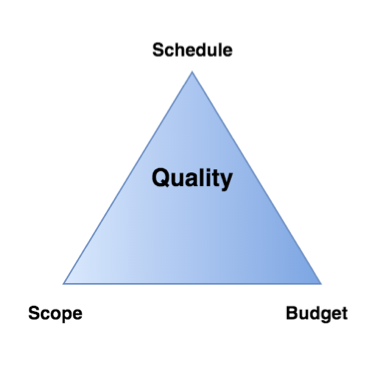
\includegraphics[width=6cm]{./img/Picture1}
  \caption{Triple Constraint Triangle}
  \label{Figure:figex}
\end{figure}


According to the triple constraint triangle above, the constraints that may delay the progress of this project are listed as follows:

\textbf{Schedule}: The duration of the project is only three months, so it is necessary to have a time management plan to ensure the project can be accomplished on time.

\textbf{Budget}: There is no budget available for this project. As such, it may restrict the access to some open datasets, because some open APIs require users to pay for more operations.

\textbf{Scope}: Due to the limitations of time and budget, the scope of this project is to meet basic requirements to complete this project on time and within budget limits.


\section{Project Methodology}

The Iterative and Incremental development model will be employed for the development of this project. In this model, the project is designed, implemented and tested incrementally until the product is finished. Also, it involves both development and maintenance. The project is defined as completed when it satisfies all of its requirements. Following this model, this project will be developed step by step. 


Figure 3.2 illustrates that the development lifecycle of this model is divided into three stages. The first stage is initial planning, which compromises the problem identification, system and requirements analysis, and system design. Then, the second stage is decomposed into some build cycles, which is designed and built separately. Each incremental build consists of the detailed design, implementation, testing and evaluation \cite{4_houston_2011}. Each build is delivered to the clients until the complete product is delivered. In this way, developers can obtain regular feedback throughout the whole lifecycle and avoid a long development time. Once all requirements are met, the final stage is to deploy the system.

\begin{figure}[H]
  \centering
  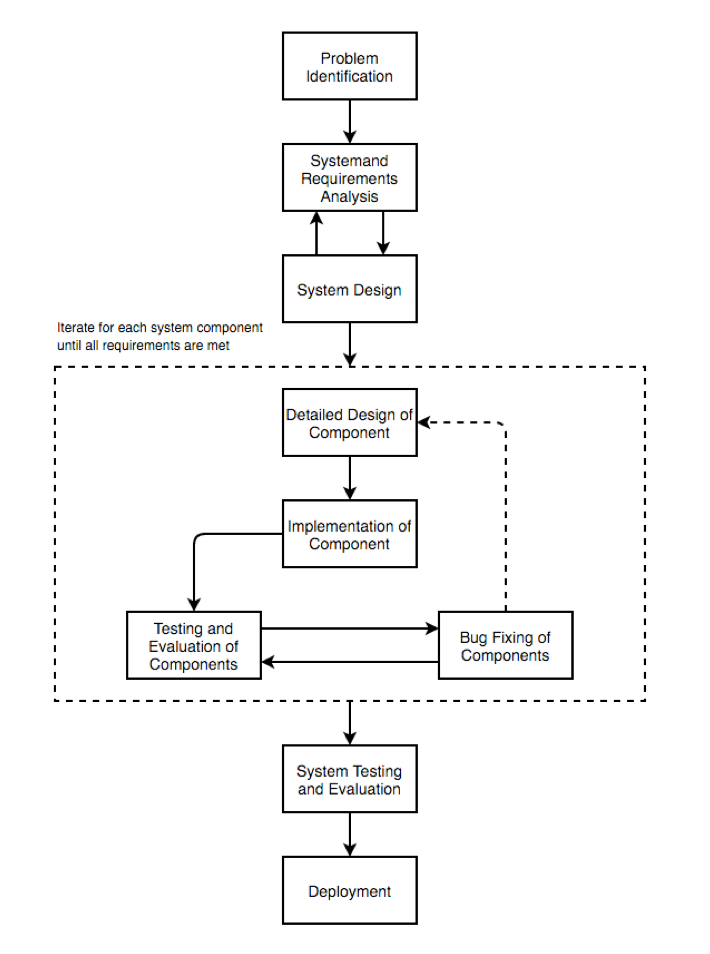
\includegraphics[width=12cm]{./img/Picture2}
  \caption{The Iterative and Incremental Development Model}
  \label{Figure:figex}
\end{figure}


\section{Time Management}

As mentioned above, the schedule is one of three constraints that hold the key to high-quality products. Hence, it is important to have a time management to ensure this project can be completed on time and achieve all user requirements.  Figure 3.3 is a Gantt chart, which includes all tasks and timings for this project. It can help distribute estimated effort to specific tasks across the duration of this project.

\begin{figure}[H]
  \centering
  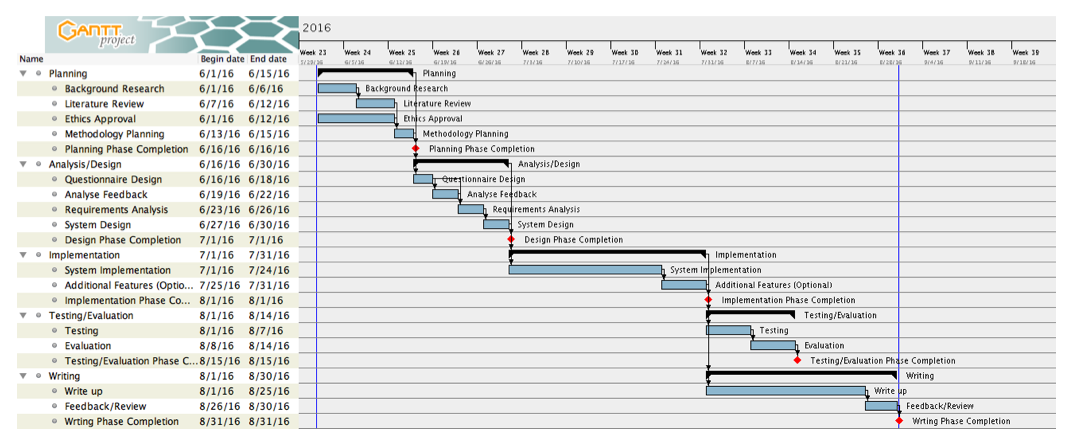
\includegraphics[width=15cm]{./img/Picture3}
  \caption{Gantt Chart}
  \label{Figure:figex}
\end{figure}

\textbf{Phase 1: Planning (2 Weeks)}

The first phase is project planning. In this phase, the background research will be conducted, which will focus on the general topic, open data, data visualisation and the relevant implementation technologies or tools. Then, the literature review about the application of open data and data visualisation in educational choices will be conducted to identify research questions, project aims and objectives. Afterwards, application documents will be submitted to ERGO committee to apply for the ethical approval. Finally, the methodology and schedule of this project will be planned.

\textbf{Phase 2: Analysis/Design (2 Weeks)}

The second phase is about requirements analysis and system design. Firstly, a questionnaire will be designed to identify factors influencing international students’ decision-making process for higher education in the UK. Based on the results of the survey, user requirements will be analysed and identified. Meanwhile, it is necessary to search for or collect relevant open datasets that reflect those factors. Afterwards, the detailed system requirements including functional and non-functional requirements will be derived from requirements analysis.

\textbf{Phase 3: Implementation (4 Weeks)}

The implementation phase is divided into two parts. The first part is system implementation, which is implemented using the technologies or tools analysed in Phase 1 and adhere to the proposed system design. The second part, which is optional is to add additional features according to users’ feedback during each incremental build. Also, this phase will overlap with phase 2 and phase 4, as all system requirements will be implemented and tested iteratively and incrementally in the development lifecycle.

\textbf{Phase 4: System Testing/ Evaluation (2 Weeks)}

In this phase, system testing, including black box and white box tests will be carried out to test the functional requirements and validate the non-functional requirements. Afterwards, the resulting web application and the whole process will be evaluated.

\textbf{Phase 5: Dissertation Writing (4 Weeks)}

This final phase is to write up the dissertation and modify it based on supervisor’s feedback. This phase and phase 4 will start at the same time as the implementation phase is completed.



\section{Risk Analysis and Management}

Risk analysis and management process is a significant step in preparation for potential risks that can occur within any software project. It can ensure any software project can be accomplished smoothly and successfully. Therefore, it is important to identify and analyse potential risks before they occur, and find appropriate measures to avoid and manage them \cite{boehm1991software}.


\subsection{Risk Identification}

The first step is to identify potential risks that can affect the success of the project. Table 3.1 provides an overview of all identified risks that can occur in this project based on Boehm's \cite{boehm1991software} prioritized top-ten list of software risks items.


\begin{table}[H]
\centering
\caption{Risk Identification}
\label{my-label}
\begin{tabular}{|p{3cm}|p{5cm}|p{5cm}|}
\hline
\textbf{Category}              & \textbf{Risk Item}                       & \textbf{Description}                                                                      \\ \hline
Personnel management risks     & Personnel shortfalls                     & Illness and other personal issues delay the completion of the project                     \\ \hline
Schedule and timing            & Unrealistic schedules and budgets        & Project cannot complete on time due to incorrectly estimated development time and budget  \\ \hline
System and functionality       & Developing the wrong software functions  & Development of software functions cannot meet users’ requirements                         \\ \cline{2-3} 
                               & Developing the wrong user interface      & Inadequate design of user interface and difficulties in usability and accessibility       \\ \hline
Requirement management         & Gold plating                             & Development of  unnecessary functions or features that not asked for by users             \\ \cline{2-3} 
                               & Continuing stream of requirement changes & Uncontrolled and unpredictable changes in system requirements or design                   \\ \hline
Resource usage and performance & Real-time performance shortfalls         & Poor system performance compromise the functionality or lead system failure               \\ \cline{2-3} 
                               & Straining computer-science capabilities  & Inability to implement the system due to lack of relevant technical solutions or datasets \\ \hline
\end{tabular}
\end{table}


\subsection{Risk Analysis}


The second step to evaluate the level and the severity of each risk in combination with the occurrence probability. Sommerville \cite{5_sommerville_2011} suggested a standard to describe the seriousness of the risks as follow:

1.	Probability: The probability of the risk might be assessed as very low (10\%), low (10-25\%), moderate (25-50\%), high (50-70\%), or very high (75\%).

2.	Effect: The effects of the risk might be assessed as catastrophic (threaten the survival of the project), serious (would cause major delays), tolerable (delays are within allowed contingency), or insignificant.

Table 3.2 displays the analysis of potential risks in this project, including their effects, occurrence probabilities and risk levels. 

\begin{table}[H]
\centering
\caption{Risk Analysis}
\label{my-label}
\begin{tabular}{|p{4cm}|p{3cm}|p{3cm}|p{3cm}|}
\hline
\textbf{Risk Item}                       & \textbf{Probability} & \textbf{Effect} & \textbf{Risk Level} \\ \hline
Personnel shortfalls                     & 10\%                 & Tolerable       & Low                 \\ \hline
Unrealistic schedules and budgets        & 70\%                 & Serious         & High                \\ \hline
Developing the wrong software functions  & 50\%                 & Catastrophic    & Moderate            \\ \hline
Developing the bad user interface        & 50\%                 & Catastrophic    & Moderate            \\ \hline
Gold plating                             & 40\%                 & Tolerable       & Moderate            \\ \hline
Continuing stream of requirement changes & 20\%                 & Tolerable       & Low                 \\ \hline
Real-time performance shortfalls         & 60\%                 & Serious         & High                \\ \hline
Straining computer-science capabilities  & 70\%                 & Serious         & High                \\ \hline
\end{tabular}
\end{table}

\subsection{Risk Management}

The final step to develops strategies to manage these potential risks. According to Sommerville \cite{5_sommerville_2011}, catastrophic risks should always be considered, as should all serious risks that have more than a moderate probability of occurrence. Therefore, mitigation strategies of identified risks are suggested in Table 3.3 to ensure that all risks are limited to minimum danger for the project.

\begin{table}[H]
\centering
\caption{Risk Management}
\label{my-label}
\begin{tabular}{|p{4cm}|p{10cm}|}
\hline
\textbf{Risk Item}                       & \textbf{Mitigation Strategy}                                                                               \\ \hline
Personnel shortfalls                     & 1. Try to work ahead of the schedule to have a time buffer                                             \\
                                         & 2. Work on weekends to catch up the delay                                                              \\ \hline
Unrealistic schedules and budgets        & 1. Divide the project into small tasks and establish specific phased targets                           \\
                                         & 2. Arrange weekly meeting with supervisor to discuss tasks, difficulties and challenges                \\ \hline
Developing the wrong software functions  & 1. Design the questionnaire carefully and scientifically to cover all requirements that users may need \\
                                         & 2. Analyse and design the requirements thoroughly                                                      \\
                                         & 3. Arrange weekly meeting with supervisor to discuss the requirements                                  \\ \hline
Developing the wrong user interface      & 1. Arrange weekly meeting with supervisor to discuss the interface and design                          \\
                                         & 2. Invite friends or peers to experience the interface and design, and ask for advice or suggestions   \\ \hline
Gold plating                             & 1. Stick strictly to the user requirements                                                             \\
                                         & 2. Focus on functionality first, then on the design                                                    \\ \hline
Continuing stream of requirement changes & 1. Design the questionnaire carefully and scientifically to cover all requirements that users may need \\
                                         & 2. Analyse and design the requirements thoroughly to avoid later changes                               \\ \hline
Real-time performance shortfalls         & 1. Choose appropriate technologies or tools to implement this project                                  \\
                                         & 2. Test and evaluate regularly to solve bugs and optimize the code                                     \\ \hline
Straining computer-science capabilities  & 1. Choose suitable technologies or tools and available datasets to implement this project              \\
                                         & 2. Ask friends for help or ask questions on forums, like stackoverflow.com                             \\ \hline
\end{tabular}
\end{table}


\section{Summary}
This chapter outlines information on project management. The triple constraint triangle, which consists of schedule, budget and scope are used to identify the project constraints. Then, the project methodology, iterative and incremental development model is introduced to explain how this project is developed. Afterwards, a Gantt chart is used to explain how the tasks and timings are managed among the phases of this project. Finally, potential risks, like personnel shortfalls are identified, and mitigation strategies of these risks are outlined to ensure the success of this project.

%% ----------------------------------------------------------------
%% Analysis.tex
%% ---------------------------------------------------------------- 

\chapter{System Analysis} \label{Chapter:System Analysis}

This chapter will focus on the system analysis. Firstly, it will identify the stakeholders of this system. Then, it will introduce a survey used for identifying significant factors influencing the higher education destination choices in the UK and analyse the survey result to identify user requirements. Eventually, this chapter will present the functional requirements and non-functional requirements of this system.


\section{Stakeholders Identification
}

Sommerville \cite{5_sommerville_2011} defined stakeholders are people or organizations who will be affected by the system and who have a direct or indirect influence on the system requirements. Hence, it is necessary to identify stakeholders that are associated with this system. 

The stakeholders of this system will be international students who want to decide destination universities or cities for their higher education in the UK or other people who want to obtain relevant information on higher education in the UK. They can use this system to search for and view information on different cities and universities to help their decision-making process for higher education in the UK.

\section{Survey Design and Analysis
}
In this project, a survey was developed to identify key factors in international students’ decision-making process and analyse the system requirements. This section will firstly introduce the design of the survey and then analyse the results of the survey.


\subsection{Survey Design
}

The survey design was based on the analysis in the section 2.1.1. The respondents of the survey were international students who planned to study in the UK for their higher education. In order to carry out this survey, an online questionnaire hosted in iSurvey was used and distributed to the respondents via emails. The online questionnaire consists of two sections and fifteen questions in total. Section 1 would ask respondents some questions about their educational background, while section 2 used a Likert scale, ranging from no influence to strong influence, to gather their opinions on factors influencing their destination choices for higher education. The online questionnaire can be found in Appendix A.


\subsection{Results Analysis
}

\textbf{Part 1: Profiles of Respondents}

This part will discuss the profiles of 107 respondents in this survey. Figure 4.1 and Figure 4.2 show 64.7\% of respondents continued to pursue their master’s degree in the UK after graduating from universities in their home countries. Besides, 5.6\% of respondents obtained their college diplomas, and 3.7\% of respondents obtained their first master’ degrees before studying in the UK. On the other hand, 25.2\% of respondents choose to study in the UK for their bachelors’ degrees after graduating from high schools.

\begin{figure}[H]
  \centering
  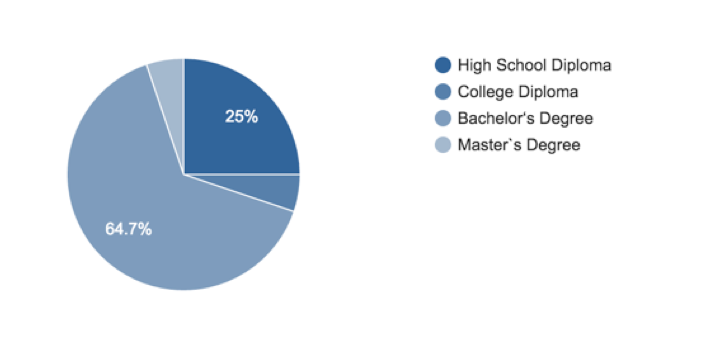
\includegraphics[width=12cm]{./img/Picture4}
  \caption{Highest Level of Education Qualification}
  \label{Figure:figex}
\end{figure}

\begin{figure}[H]
  \centering
  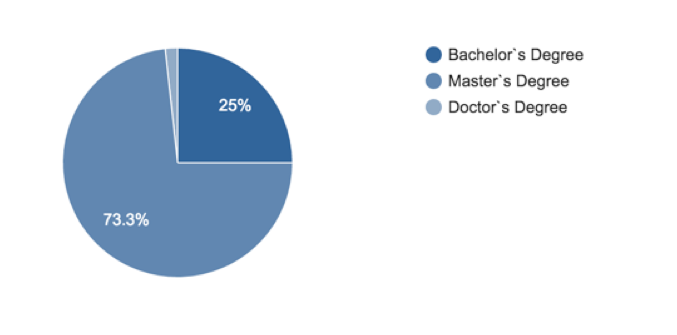
\includegraphics[width=12cm]{./img/Picture5}
  \caption{Level of Education Qualification Pursuing in the UK}
  \label{Figure:figex}
\end{figure}

Figure 4.3 shows most (83.2\%) of respondents choose to study in universities in England (except Greater London), while respondents who choose to study in Greater London, Wales and Scotland only accounted for 6.5\%, 5.6\% and 4.7\% respectively. The main reason was that England (except Greater London) had more universities and lower living expenses compared with Greater London and closer distance to London compared with Wales and Scotland. 

\begin{figure}[H]
  \centering
  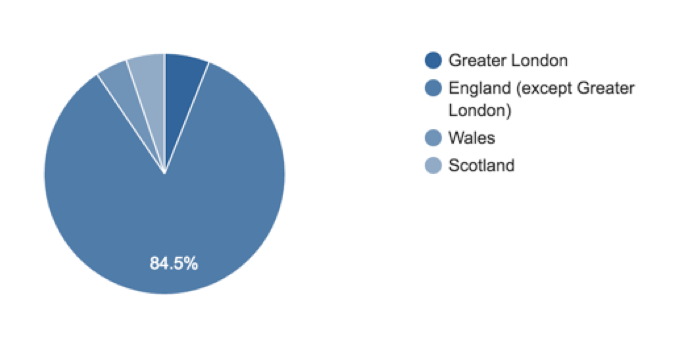
\includegraphics[width=11cm]{./img/Picture6}
  \caption{The Location of University}
  \label{Figure:figex}
\end{figure}

\textbf{Part 2: Perception of the Respondents}

This part will focus on the perception of respondents on different factors in their higher education destination choices. The discussion and analysis in this part will provide a great understanding of factors influencing international student’s higher education destination choices in the UK.

Table 4.1 provides the overview of the perception of respondents regarding what factors have impacts on their destination choices in the UK. It is evident that cost and environment strongly influenced the respondents’ destination higher education choices, and university ranking was considered as a very influential factor in their destination-making process. By contrast, recommendations, employment rate and entry requirements had moderate influences on the respondents’ destination choices, and the least influential factor was international student population. 

\begin{table}[H]
\centering
\caption{Factors Influencing Destination Choices in the UK
}
\label{my-label}
\begin{tabular}{|p{4cm}|c|c|c|c|c|p{2cm}|p{3cm}|}
\hline
                                                                          & \textbf{1} & \textbf{2} & \textbf{3} & \textbf{4} & \textbf{5} & \textbf{Weighted Mean} & \textbf{Interpretation} \\ \hline
University Ranking                                                        & 0          & 1          & 24         & 46         & 36         & 4.09                   & Very Influential        \\ \hline
Cost (tuition fee, living cost, travel cost, etc.)                        & 2          & 0          & 8          & 26         & 71         & 4.53                   & Strongly Influential    \\ \hline
Environment (climate, city size, city location, crime rate of city, etc.) & 2          & 2          & 5          & 20         & 78         & 4.58                   & Strongly Influential    \\ \hline
Recommendations (Word of mouth)                                           & 1          & 22         & 53         & 26         & 5          & 3.11                   & Somewhat Influential    \\ \hline
Entry requirements                                                        & 1          & 17         & 47         & 38         & 4          & 3.24                   & Somewhat Influential    \\ \hline
Employment rate                                                           & 2          & 15         & 44         & 29         & 17         & 3.41                   & Somewhat Influential    \\ \hline
International Student Population                                          & 28         & 51         & 22         & 4          & 2          & 2.07                   & Slightly Influential    \\ \hline
\end{tabular}
\end{table}

In order to get more details about these key factors, some specific questions were included in the online questionnaire. Table 4.2 presents the perception of respondents about university rankings. Because of the reputations and impacts, Times Higher Education university ranking and QS university ranking were considered to be more influential on respondents’ higher education destination choices, even if all rankings about universities in the UK were regarded as very influential factors concerning university rankings.


\begin{table}[H]
\centering
\caption{Influence of Different University Rankings
}
\label{my-label}
\begin{tabular}{|p{4cm}|c|c|c|c|c|p{2cm}|p{3cm}|}
\hline
                                                                   & \textbf{1} & \textbf{2} & \textbf{3} & \textbf{4} & \textbf{5} & \textbf{Weighted Mean} & \textbf{Interpretation} \\ \hline
Guardian University Ranking                                        & 3          & 1          & 25         & 47         & 31         & 3.95                   & Very Influential        \\ \hline
Times Higher Education University Ranking                          & 0          & 4          & 11         & 30         & 62         & 4.4                    & Very Influential        \\ \hline
QS University Ranking                                              & 0          & 1          & 14         & 31         & 61         & 4.45                   & Very Influential        \\ \hline
US News Global Universities Ranking                                & 2          & 46         & 35         & 20         & 4          & 2.79                   & Somewhat Influential    \\ \hline
Research Excellence Framework (REF)                                & 1          & 3          & 16         & 52         & 35         & 4.09                   & Very Influential        \\ \hline
The Complete University Guide Ranking (CUG)                        & 2          & 4          & 45         & 45         & 11         & 3.55                   & Very Influential        \\ \hline
Academic Ranking of World Universities (Shanghai JiaoTong Ranking) & 67         & 24         & 9          & 4          & 3          & 1.62                   & Slightly Influential    \\ \hline
\end{tabular}
\end{table}

Table 4.3 illustrates the perception of respondents regarding different expenses, such as tuition fees, living costs and travel costs. It was evident that travel expenses had fewer impacts on the respondents’ decision-making process for higher education, compared with tuition fees and living costs. 

\begin{table}[H]
\centering
\caption{Influence of Different Expenses}
\label{my-label}
\begin{tabular}{|p{4cm}|c|c|c|c|c|p{2cm}|p{3cm}|}
\hline
            & \textbf{1} & \textbf{2} & \textbf{3} & \textbf{4} & \textbf{5} & \textbf{Weighted Mean} & \textbf{Interpretation} \\ \hline
Tuition fee & 1          & 1          & 3          & 31         & 71         & 4.58                   & Strongly Influential    \\ \hline
Living cost & 1          & 1          & 8          & 29         & 68         & 4.51                   & Strongly Influential    \\ \hline
Travel cost & 3          & 27         & 51         & 23         & 3          & 2.96                   & Somewhat Influential    \\ \hline
\end{tabular}
\end{table}

Table 4.4 shows the perception of the respondents on different environmental factors. Information on the safety and location of the city were regarded as two strongly influential factors in the respondents’ decision-making process. Moreover, other information on cities, such as size, location and infrastructure were also considered in their decision making.


\begin{table}[H]
\centering
\caption{Influence of Different Environmental Factors
}
\label{my-label}
\begin{tabular}{|p{4cm}|c|c|c|c|c|p{2cm}|p{3cm}|}
\hline
                                                               & \textbf{1} & \textbf{2} & \textbf{3} & \textbf{4} & \textbf{5} & \textbf{Weighted Mean} & \textbf{Interpretation} \\ \hline
Campus environment                                             & 1          & 2          & 54         & 41         & 9          & 3.5                    & Very Influential        \\ \hline
Climate (weather)                                              & 2          & 3          & 9          & 50         & 43         & 4.2                    & Very Influential        \\ \hline
Safety of the city                                             & 1          & 1          & 9          & 33         & 63         & 4.46                   & Strongly Influential    \\ \hline
City size                                                      & 3          & 0          & 36         & 23         & 45         & 4                      & Very Influential        \\ \hline
City location (geographic proximity to capital city or London) & 0          & 1          & 14         & 19         & 73         & 4.53                   & Strongly Influential    \\ \hline
City infrastructure (airport, railway station, etc.)           & 2          & 8          & 21         & 20         & 56         & 4.12                   & Very Influential        \\ \hline
\end{tabular}
\end{table}


Table 4.5 provides the perception of the respondents on recommendations or word-of-mouth. It can be seen that recommendations from agents and official website were more influential than those from the respondents’ parents and friends.

\begin{table}[H]
\centering
\caption{Influence of Recommendations From Different People
}
\label{my-label}
\begin{tabular}{|p{4cm}|c|c|c|c|c|p{2cm}|p{3cm}|}
\hline
                            & \textbf{1} & \textbf{2} & \textbf{3} & \textbf{4} & \textbf{5} & \textbf{Weighted Mean} & \textbf{Interpretation} \\ \hline
Parents/Relatives           & 2          & 5          & 17         & 55         & 28         & 3.95                   & Very Influential        \\ \hline
Friends                     & 2          & 4          & 18         & 65         & 18         & 3.87                   & Very Influential        \\ \hline
Agents                      & 3          & 7          & 13         & 31         & 53         & 4.15                   & Very Influential        \\ \hline
University official website & 2          & 4          & 9          & 29         & 63         & 4.37                   & Very Influential        \\ \hline
\end{tabular}
\end{table}


To summarize, the key factors in the international students’ decision-making process for higher education are “university ranking”, “cost” and “environment”. Therefore, information on these three factors should be contained in the system. Specifically, there is no great difference between universities rankings when the international students want to know the reputation of universities as long as these rankings are about universities in the UK. In term of costs, the international students pay much more attention to tuition fees and living expenses, so information on these two types of costs should be provided in this system. Besides, the information on safety and location of cities should also be included in the system to provide information on the environment for international students’ higher education destination choices in the UK. 

\section{User Requirements
}

Based on the analysis above, we can identify user requirements that the stakeholders expect in this system in Table 4.6.

\begin{table}[H]
\centering
\caption{User Requirements of This System
}
\label{my-label}
\begin{tabular}{|p{2cm}|p{11cm}|}
\hline
\textbf{Identifier} & \textbf{User Requirement}                                                                                                               \\ \hline
UREQ1               & As an international student, I want to search for the universities and programs in the UK.                                              \\ \hline
UREQ2               & As an international student, I want to know the ranking of a certain university.                                                        \\ \hline
UREQ3               & As an international student, I want to know the tuition fee in a certain university or city.                                            \\ \hline
UREQ4               & As an international student, I want to know the living expense in the city that a certain university is located in                      \\ \hline
UREQ5               & As an international student, I want to know the employment rate of a certain program                                                    \\ \hline
UREQ6               & As an international student, I want to know the entry requirement of a certain program                                                  \\ \hline
UREQ7               & As an international student, I want to know the campus environment of a certain university.                                             \\ \hline
UREQ8               & As an international student, I want to know the location of a certain university.                                                       \\ \hline
UREQ9               & As an international student, I want to know the geographic proximity of this university to capital city or London.                      \\ \hline
UREQ10              & As an international student, I want to know the size of the city that a certain university is located in.                               \\ \hline
UREQ11              & As an international student, I want to know the climate or weather of the city that a certain university is located in.                 \\ \hline
UREQ12              & As an international student, I want to know the information on criminality in the city that a certain university is located in.         \\ \hline
UREQ13              & As an international student, I want to know the infrastructure in the city that a certain university is located in.                     \\ \hline
UREQ14              & As an international student, I want to share information on a certain university or program to get some advice from parents or friends. \\ \hline
UREQ15              & As an international student, I want to know some information on a certain university or program from its official website.              \\ \hline
\end{tabular}
\end{table}


\section{System Requirements
}

\subsection{Functional Requirements
}

The functional requirements of this system are derived from the above user requirements. Table 4.7 displays the functional requirements with their descriptions. Due to time constraints, the requirements are categorized into high, medium and low. The implementation will focus the requirements with high priority to achieve the system’s main objectives.

\begin{table}[H]
\centering
\caption{Functional Requirements of This System
}
\label{my-label}
\begin{tabular}{|p{2cm}|p{3cm}|p{1.5cm}|p{7cm}|}
\hline
\textbf{Identifier} & \textbf{Related User Requirement}         & \textbf{Priority} & \textbf{Description}                                                                                                              \\ \hline
FRQ1                & UREQ1, UREQ3, UREQ4, UREQ5, UREQ6, UREQ15 & High              & The system shall allow users to search for universities or programs and offer users relevant information on them.                 \\ \hline
FRQ2                & UREQ2                                     & High              & The system shall allow users to know the ranking of a certain university.                                                         \\ \hline
FRQ3                & UREQ7, UREQ8, UREQ9                       & High              & The system shall allow users to know the campus environment, the location and the geographic proximity of a certain university    \\ \hline
FRQ4                & UREQ10                                    & Medium            & The system shall allow users to know the size of the city that a certain university is located in                                 \\ \hline
FRQ5                & UREQ11                                    & High              & The system shall allow users to know the climate or weather of the city that a certain university is located in.                  \\ \hline
FRQ6                & UREQ12                                    & High              & The system shall allow users to know the information  on criminality in the city that a certain university is located in is safe. \\ \hline
FRQ7                & UREQ13                                    & High              & The system shall allow users to know the infrastructure in the city that a certain university is located in.                      \\ \hline
FRQ8                & UREQ14                                    & Medium            & The system shall allow users to share information on a certain university or program to get some advice from parents or friends.  \\ \hline
\end{tabular}
\end{table}


\subsection{Non-functional Requirements
}

Apart from functional requirements, the non-functional requirements should be taken into consideration during the design and implementation stages. Table 4.8 displays the non-functional requirements that should be complied with to build a high-quality system.

\begin{table}[H]
\centering
\caption{Non-functional Requirements of This System}
\label{my-label}
\begin{tabular}{|p{2cm}|p{3cm}|p{8cm}|}
\hline
\textbf{Identifier} & \textbf{Type}   & \textbf{Description}                                                                                                             \\ \hline
NRQ1                & Usability       & The interface of this system should be well structured or easy to learn and understand.                                          \\ \hline
NRQ2                & Usability       & The interface of this system should be responsive or be able to adjust itself on different devices (PC, smartphones and tablets) \\ \hline
NRQ3                & Accessibility   & The design of this system should comply with Web accessibility standards provided by W3C.                                        \\ \hline
NRQ4                & Availability    & The system should be available  95\% of the time for any day.                                                                    \\ \hline
NRQ5                & Compatibility   & The system should be compatible with commonly-used web browsers (Chrome, Firefox, IE and Safari)                                    \\ \hline
NRQ6                & Maintainability & The code of this system should be easy to maintain. The usage of MVVM pattern can ensure this system is easy to maintain.                                                                              \\ \hline
%NRQ7                & Performance     & The system should be able to handle ten requests per second.                                                                     \\ \hline
\end{tabular}
\end{table}


\section{Summary}
This chapter provides information on the system analysis. It consists of the stakeholders of this system, the user requirements, the system requirements (functional and non-functional requirements). Besides, the survey designed for identifying key factors in international students’ decision-making process is introduced and analysed to determine the user requirements of this system.


%% ----------------------------------------------------------------
%% Design.tex
%% ---------------------------------------------------------------- 

\chapter{System Design} \label{Chapter:System Design}

System design is a fundamental process of the software development that defines the architecture, the components and the interface of a system to satisfy specific user requirements. This chapter will firstly describe the sources of open datasets and how they will be utilized in this system. Then it will detailedly discuss the system design based on the background research and the system. Finally, the user interface design of this system will be introduced using some typical wireframes drawings.

\section{Open Datasets}
After identifying the functional requirements, it is necessary to search for or collect relevant open datasets and use them in data visualisation. Due to time constraints, public APIs (Application program interfaces) become the first choices of this system. The advantage of APIs is that the developers do not need to pre-process data and design database, which can save much time in the software development lifecycle. Also, the real-time access to APIs can ensure that the latest data can be obtained. However, it may be a problem that some open APIs are likely to restrict unlimited access or require users to pay for more operations.

\subsection{Unistats API}

Unistats API is an open API provided by Higher Education Statistics Agency (HESA). This API provides comparable sets of information about university courses in the UK, such as course mode, tuition fees and living expenses. Moreover, it provides the details of the location of universities or courses, including the latitude and longitude. Therefore, this API was used to provide international students with information on universities and courses.


\subsection{Google Maps API
}

Google Maps provides some map APIs that allow the developers to add different functions to the embedded Google Map on the web pages. In this system, Google Maps Distance Matrix API was used to estimate travel time and distance between universities and several metropolises, like London and Edinburgh. Besides, Google Map Places API was used to provide information about infrastructure around universities.


\subsection{OpenWeatherMap API
}

Although the historical weather data would offer a better understanding of weather in cities, it is hard to find available open datasets or free open APIs about the historical weather of cities in the UK. Most open datasets, like Met Office, only provide historical weather data of observation stations instead of that of cities. As a result, the information about weather provided in this system was the weather forecast for next hours and next 14 days, and the data came from OpenWeatherMap API.

\subsection{Police API
}

Police.uk provides a Police API that gives the public free access to open data about crime and policing in England, Wales and Northern Ireland. Specifically, the Police API allows the public to retrieve data about crime or policing within different locations or categories. Hence, the police API was used in this system to provide international students with detailed information on criminality or safety of cities. 

\subsection{THE University Ranking Table 
}

Due to the lack of related open APIs, the dataset about university ranking was from THE university ranking tables, which included some ranking criteria, such as teaching quality and student experience.  The dataset was originally manipulated using Open Refine. After data manipulation, it was saved as a CSV file and displayed in a table.

\section{Architecture Design
}


The architecture design is a process that describes the structure, behaviour and more views of a system and it has a great impact on the performance, robustness, distributability, and maintainability of a system \cite{5_sommerville_2011}. 


AngularJS, a kind of front-end JavaScript framework, is used to implement this system. More in detail, the overall architecture of this system is the model-view-viewmodel (MVVM) pattern. Though a server-side proxy is used in this system to send proxied front-end requests to Unistats API, it is only used for Unistats API and not the core part of the system architecture. Therefore, the server-side proxy is not present in the architecture design in order to make it easy to understand. MVVM pattern helps separate business logic (model) from the UI (view) using the view model, so it allows the developers to write better organized, and therefore more maintainable system. As Figure 5.1 shows, the MVVM pattern has three logical components (model, view and view model), which are interrelated and interact with each other. The detailed interaction between these three components will be explained in the following section.
\begin{figure}[H]
  \centering
  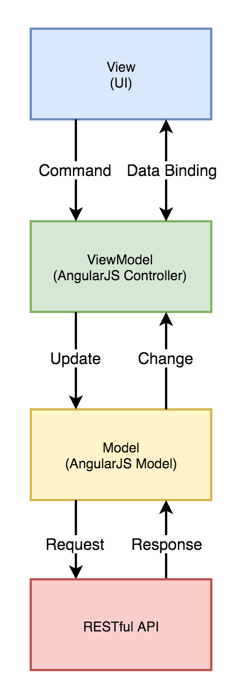
\includegraphics[width=4cm]{./img/Picture7}
  \caption{System Architecture}
  \label{Figure:figex}
\end{figure}



\section{Detailed Design}
\subsection{Use Case Diagram}
Figure 5.2 is a use case diagram shows the overview of the functional requirements provided in this system and the interactions between the users and the system. The users of this system are international students who want to get information about universities and cities for their higher education destination choices. It is noticeable that these use cases have include or extend relationships with each other. Particularly, “View University\&Course Part” and other five use cases are included in “Search universities and courses”, which means that all these six use cases can only be accomplished after searching universities and courses.

\begin{figure}[H]
  \centering
  \includegraphics[width=15cm]{./img/Picture8}
  \caption{Use Case Diagram}
  \label{Figure:figex}
\end{figure}

\subsection{Activity Diagram}
An activity diagram is a simple and intuitive representation of what happens in a workflow, what activities can be done in parallel, and whether there are alternative paths through the workflow \cite{IBM}. Therefore, an activity diagram can help understand the workflow of activities while using this system. As shown in Figure 5.3, it is clear that the workflow of this system is simple and straightforward, which makes it easy for the users to understand and use this system. Apart from the activities in the following figure, the users also can select different months and different kinds of infrastructure in criminality and infrastructure part respectively. 
 


\begin{figure}[H]
  \centering
  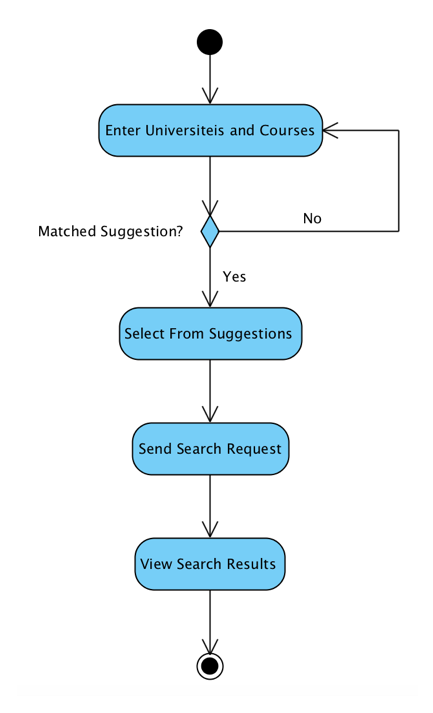
\includegraphics[width=6cm]{./img/Picture9}
  \caption{Activity Diagram
}
  \label{Figure:figex}
\end{figure}



\subsection{Sequence Diagram}
The purpose of a sequence diagram is to show interactions and communications between the objects of a system in time sequence \cite{IBM2}. Figure 5.4 presents a sequence diagram that is used to present how the components of MVVM pattern interact with each other when the users interact with the view.

\textbf{Model}: The Model, which refers to the controllers in AngularJS, is responsible for sending requests to various RESTful APIs and return related data to the view model.

\textbf{View}: The View, which refers to the user interface, is responsible for receiving commands from users and displaying the data that is supplied by the view model as result. 

\textbf{View Model}: The View Model is responsible for presenting data from the model, receiving data change of view and change the model.



\begin{figure}[H]
  \centering
  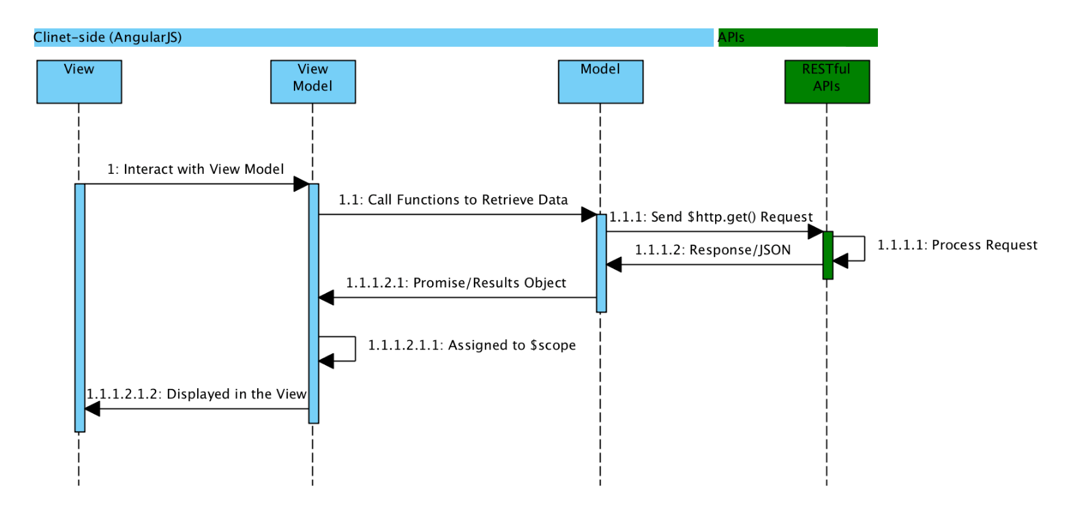
\includegraphics[width=16cm]{./img/Picture10}
  \caption{Sequence Diagram of MVVM Pattern}
  \label{Figure:figex}
\end{figure}



Moreover, Figure 5.5 is an another sequence diagram that provides information about the interactions between the browser and several open APIs used in this system. When the users send search requests via the browser, Unistats API will return data about the selected universities and courses, and the responses will be displayed on the webpage. Meanwhile, the browser will send several requests containing the geolocation data about cities, which are from Unistats API, to other open APIs. Afterwards, these APIs will return related data about cities to the browser accordingly.



\begin{figure}[H]
  \centering
  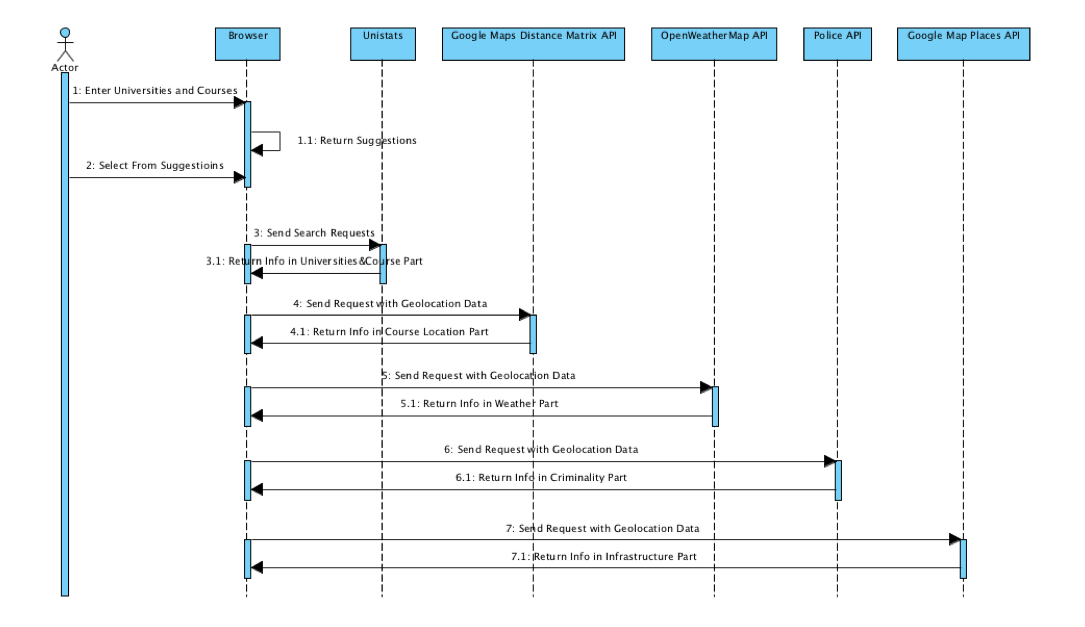
\includegraphics[width=15cm]{./img/Picture11}
  \caption{Sequence Diagram of Interaction Between Brower and Open APIs}
  \label{Figure:figex}
\end{figure}


\section{User Interface Design
}

A fundamental reality of software development is that the user interface is the system to the users \cite{ambler2000user}. Hence, the user interface is as important as the functionality that a system provides to the users. A good user interface design can make the system easy to use and understand. To ensure this system available in different devices (PC, smartphones and tablets), the responsive web design is used for the user interface of this system. In this section, some typical wireframes drawings will be used to introduce the user interface design of this system.


\subsection{Layout}

The layout of the system was the first element that should be considered in the use interface design. A well-designed layout allows users to gain insights into the functionalities of the system rapidly and intuitively. There were two sections in this system, namely university section and about section. The webpage of each section can be divided into three parts as shown in Figure 5.6. The top (1) and bottom (3) of the webpage was a navigation bar and a footer, which can offer the users quick access to the sections in this system and some additional information respectively. The middle (2) of the webpage was used to display main content of each section.


\begin{figure}[H]
  \centering
  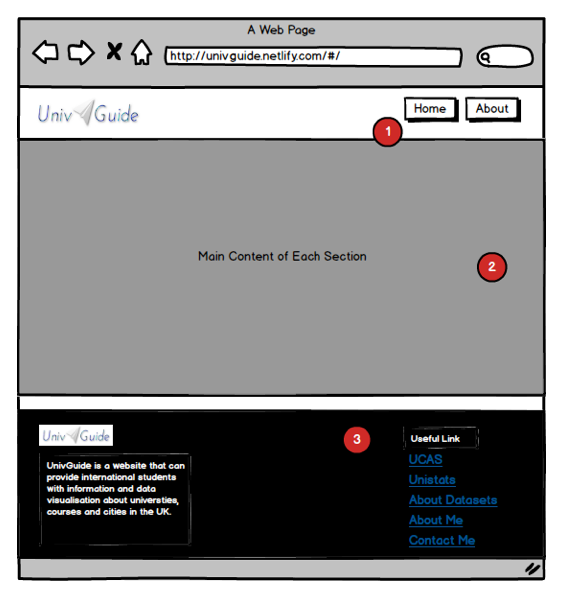
\includegraphics[width=10cm]{./img/Picture12}
  \caption{Layout}
  \label{Figure:figex}
\end{figure}



\subsection{Initial Page}
The initial page (see Figure 5.7) was designed for the users who enter this system at the first time.  It presented the overview or guide (5) of this system. Besides, the search bar (4) was placed in a prominent position because it was the most important component of this system.


\begin{figure}[H]
  \centering
  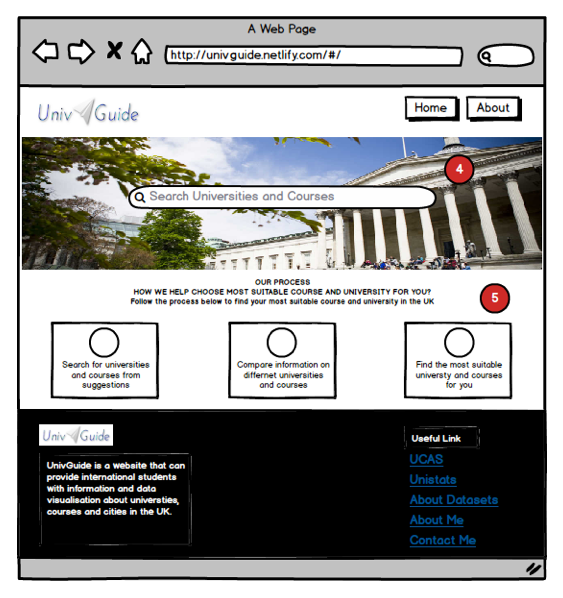
\includegraphics[width=10cm]{./img/Picture13}
  \caption{Initial Page}
  \label{Figure:figex}
\end{figure}


\subsection{University section
}

When the users search for universities or courses and select one from suggestions, the university section will replace the overview (5) of this system. The university section (see Figure 5.8) consists of search parts, namely University\&Course (6), Ranking Table (7), Course Location (8) and City Information (9). These parts are the core functionalities of this system. Specifically, University\&Course part contains information about selected universities or courses; The ranking table displays THE University Ranking; The course location part presents the location and the geographic proximity of selected universities or courses. The city information part includes information about weather, criminality and infrastructure of the cities that selected universities or courses are located in.



\begin{figure}[H]
  \centering
  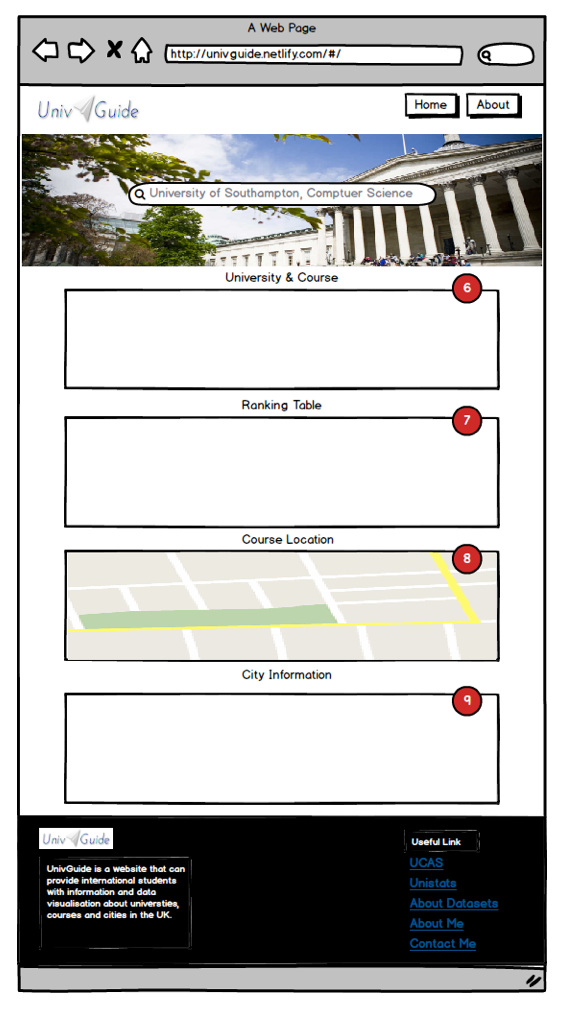
\includegraphics[width=10cm]{./img/Picture14}
  \caption{University Section}
  \label{Figure:figex}
\end{figure}



\subsection{About section
}

The about section (see Figure 5.9) provided some additional information about this system, such as the goal of this system (10), the data sources (11) and the people involved in its development (12).


\begin{figure}[H]
  \centering
  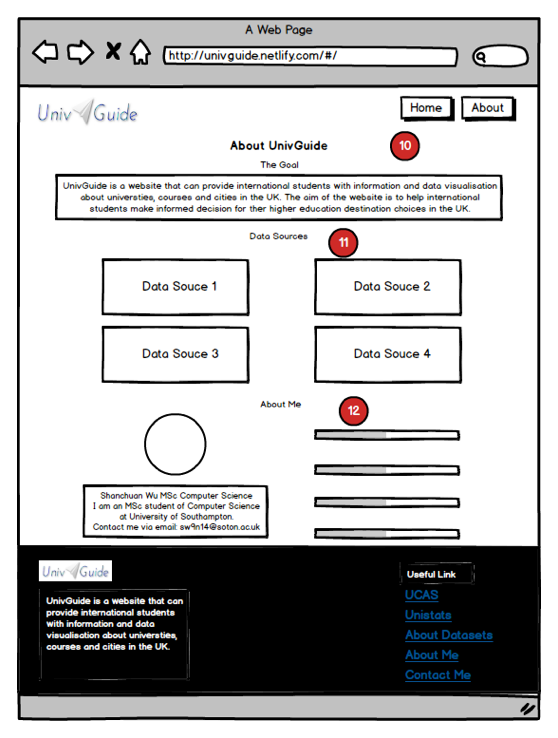
\includegraphics[width=10cm]{./img/Picture15}
  \caption{About Section}
  \label{Figure:figex}
\end{figure}



\section{Summary}

This chapter firstly provides information about the sources of open datasets and explains how they are used in this system to provide information about universities and cities in the UK. Afterwards, the detailed design of this system is introduced with some UML diagrams. At last, several wireframes drawings are presented to illustrate the prototype of user interface design. 





%% ----------------------------------------------------------------
%% Implementation.tex
%% ---------------------------------------------------------------- 

\chapter{System Implementation} \label{Chapter:System Implementation}

This chapter will give detailed information about the implementation of this system. It will start with the introduction of the implementation technologies and tools for this system. Afterwards, this chapter will explain how the main components of this system are implemented to conform to the requirement specifications.


\section{Technologies and Tools
}
Appropriate implementation technologies and tools are the keys to the success of a software system, while poor choices may cause difficulties, delays or even failure of a software system. Regarding the system analysis and design, the following technologies and tools are chosen to develop this system. 



\subsection{Programming Language}

JavaScript is chosen as the main programming language for developing this system. There are several reasons for this choice. Firstly, AngularJS is a JavaScript-based front-end framework, so it is natural to choose JavaScript as the programming language. Secondly, many third-party libraries, like D3.js, for data visualisation are written in JavaScript. Last but not the least, JavaScript, which is the most popular programming language in the world \cite{ARC}, has a big community and a variety of tutorials, which makes it easy to develop and maintain this system. 


\subsection{Development Framework}

In order to build this system rapidly and efficiently, AngularJS, a commonly-used front-end framework is chosen to develop this system. More narrowly, the framework of this system is MVVM pattern, as explained in chapter 5. This pattern allows the developers to write better organized, and therefore more maintainable system, so it a good choice for developing this system.

\subsection{User Interface}

Apart from AngularJS, some basic building technologies of the front-end development are used for the web interface design. HTML5 is used for structuring and presenting content on the web interface, and CSS3 is used for describing the presentation of a document written in HTML5.
 
\subsection{Data Visualisation}

Regarding with the objectives of this project, some data visualisation technologies are chosen to visualize open data. Highcharts.js is a charting library written in JavaScript, offering an easy way of adding interactive charts to the website web application. It is used to visualize weather data from OpenWeatherMap API and provide international students with data visualisation about the weather information of cities. 

Although highcharts.js can provide developers with a rapid way of adding charts in the web pages, it only has limited choices of charts. Hence, D3.js is also used in this system to visualize crime data from Police API. It is a JavaScript library that allows developers to build the data visualisation framework they want. Besides, the requirements analysis in chapter 4 suggests that the location of universities and the environment of cities are crucial factors influencing international students’ decision-making process. So, Google Maps JavaScript API is applied in this system to visualize the geographical information and the infrastructure of cities.


\subsection{Development Tools}

There are two main development tools used for this system. One tool is Github, a version control tool for managing this system and keeping track of the changes in code, and another one is Atom, an integrated development environment (IDE) for developing the web application of this project.

\section{System Components Implementation}

Based on the system analysis and design, some components are built to implement this system. This section will explain the main components of this system with some screenshots and necessarily codes presented. 


\subsection{Search Bar
}	
As shown in the use case diagram, most components of this system rely on the search results, so the search bar is the most important functionality of this system. The first step for the users is to search universities and courses while using this system. 

\begin{figure}[H]
  \centering
  
\includegraphics[width=15cm]{./img/Picture16}
  \caption{Search Bar}
  \label{Figure:figex}
\end{figure}

\begin{figure}[H]
  \centering
  
\includegraphics[width=6cm]{./img/Picture17}
  \caption{University Name, Course Title and Corresponding Identifiers
}
  \label{Figure:figex}
\end{figure}

In order to improve the user experience, the search bar is implemented using Algolia \cite{Alogolia} for real-time search and typo tolerance (see Figure 6.1). Another reason for using Algolia is that \$http.get() requests sent to Unistats API can only take the identifiers of universities and courses as parameters, so it is necessary to covert the users’ searching inputs (university names and course titles) to corresponding identifiers (UKPRN and KISCOURSEID) before sending those requests to Unistats API. The JSON file (see Figure 6.2) that contains university names and course titles as well as their corresponding identifiers is stored in Algolia. 








When the users enter university names and course titles, the suggestions will show up and the matched results will be highlighted. Once the suggestions are selected, the search bar will convert the inputs to their corresponding identifiers and send \$http.get() requests containing these identifiers to Unistats API. 

\subsection{University \& Course}

The University\&Course part provides some basic information about universities and courses, such as tuition fee and living expense, to help the users gain quick insights into them. Figure 6.3 shows part of information displayed in University\&Course part. 

\begin{figure}[H]
  \centering
  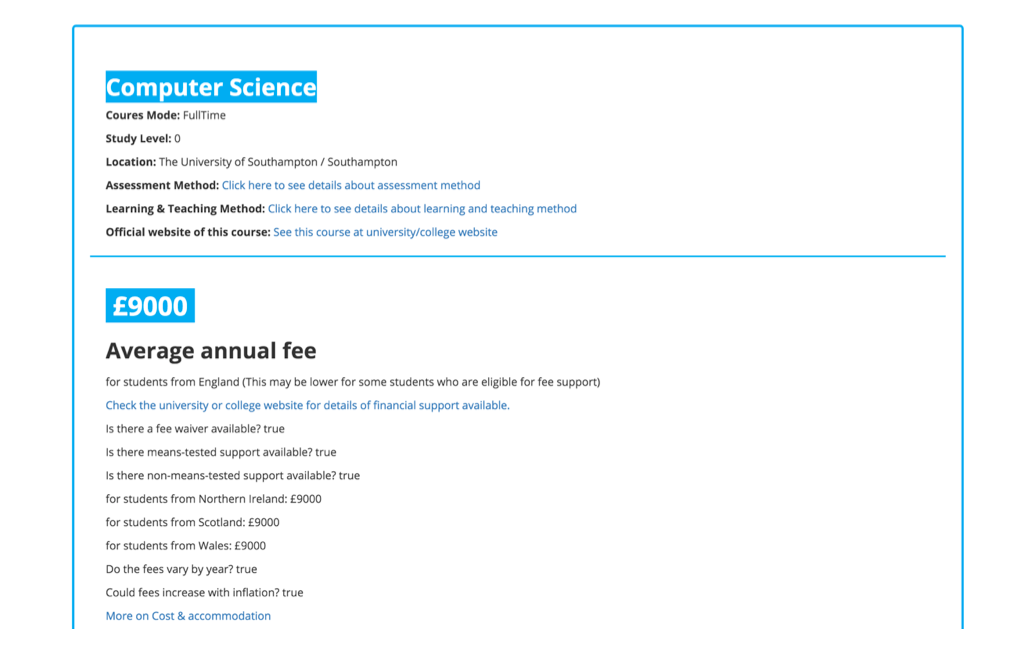
\includegraphics[width=15cm]{./img/Picture18}
  \caption{University \& Course Part}
  \label{Figure:figex}
\end{figure}


\begin{figure}[H]
  \centering
  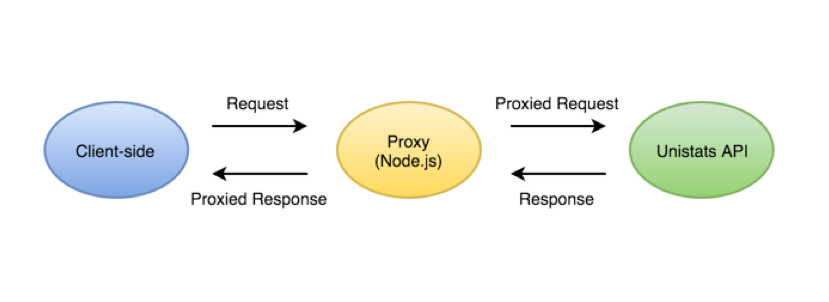
\includegraphics[width=12cm]{./img/Picture19}
  \caption{Server-side Proxy
}
  \label{Figure:figex}
\end{figure}

As discussed above, four \$http.get() requests will be sent to Unistats API to get information about the selected universities and courses, but the problem is that \$http.get() requests sent from the client side is not allowed by Unistats API. To solve this problem, Node.js is used in this system to allow these requests through a server side proxy and have the server side proxy return the data back to the client side (see Figure 6.4).

\begin{figure}[H]
  \centering
  
\includegraphics[width=15cm]{./img/Picture20}
  \caption{Client-side Requests}
  \label{Figure:figex}
\end{figure}


As shown in Figure 6.5, an endpoint (/hello) is set up to grab these four requests to the server side. The client side will send those parameters to the port of the server side after receiving the search results from the search bar. Afterwards, the server side proxy will send the proxied requests (see Figure 6.6) to Unistats API and return responses to the client side. Finally, the client-side will display the proxied responses on the webpage. 

\begin{figure}[H]
  \centering
  
\includegraphics[width=15cm]{./img/Picture21}
  \caption{Server-side Proxied Proxy
}
  \label{Figure:figex}
\end{figure}



\subsection{Ranking Table}

The ranking table (see Figure 6.7) of this system provides the users with the ranking and the score variation of all ranking criteria of universities in the UK. Moreover, the users are allowed to interact with the ranking table. For example, the users can reorder the ranking table according to different ranking criteria. 

\begin{figure}[H]
  \centering
  \includegraphics[width=15cm]{./img/Picture22}
  \caption{Ranking Table Part}
  \label{Figure:figex}
\end{figure}


\subsection{Course Location}

As mentioned in section 5.3.3, the browser will send requests containing the geolocation data (latitude and longitude) about cities to other open APIs used in this system. Therefore, the Course Location part (see Figure 6.8) can provide information about the locations of cities when the users search for universities. Assuming the user wants to search computer science in University of Southampton, the browser will send requests containing the identifiers of University of Southampton and computer science to Unistats API. Then, Unistats API will return data about computer science in University of Southampton with the geolocation data about Southampton to the browser. After receiving the geolocation data, the browser will send it to Google Map Matrix API, which is used to display the location of Southampton on the map. Also, Google Map Matrix API is used to calculate the distances and driving time between Southampton and several metropolises, like London and Manchester, which can help the users to gain an insight into the location of Southampton at ease.

\begin{figure}[H]
  \centering
  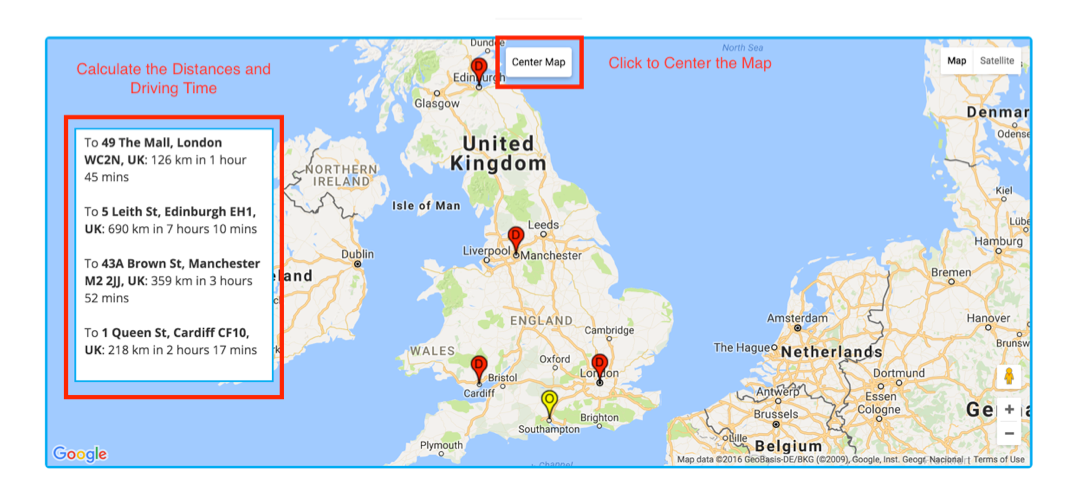
\includegraphics[width=15cm]{./img/Picture23}
  \caption{Course Location Part}
  \label{Figure:figex}
\end{figure}


\subsection{Weather}




According to the geolocation data from Unistats API, the weather part can get data about the weather in different cities from OpenWeatherMap API (see Figure 6.9) and visualize it using highchart.js (see Figure 6.10).

\begin{figure}[H]
  \centering
  
\includegraphics[width=15cm]{./img/Picture24}
  \caption{Requests Sent to OpenWeatherMap API
}
  \label{Figure:figex}
\end{figure}

\begin{figure}[H]
  \centering
  \includegraphics[width=15cm]{./img/Picture25}
  \caption{Weather Part
}
  \label{Figure:figex}
\end{figure}

Figure 6.10 presents the weather forecast in Southampton. Specifically, these two charts display the variations of temperature and precipitation in next hours and next 14 days in Southampton respectively. Moreover, the users are allowed to interact with the charts. For instance, the users can hover over the charts and see the tooltips. 




\subsection{Criminality}

The criminality part provides a map that visualizes the crime data of different cities, and this can provide a great understanding of the safety of cities. As shown in Figure 6.11, the crime data of Southampton in May 2016 is visualized in the circles of different colours and sizes, and the tooltips of the circles give the users more details about the crimes in a certain location. On the other hand, the panel on the left gives an overview of the crime data. The pie chart shows the colours and the percentages of different types of crimes and the drop-down box allows the users to select the crime data in different months.

\begin{figure}[H]
  \centering
  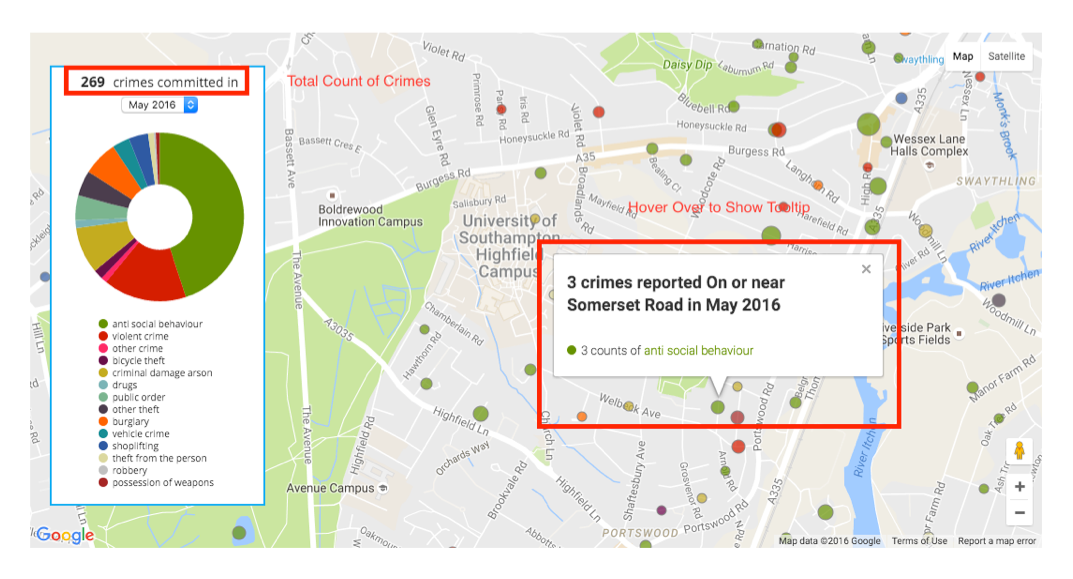
\includegraphics[width=15cm]{./img/Picture26}
  \caption{Criminality Part
}
  \label{Figure:figex}
\end{figure}


\subsection{Infrastructure}

The infrastructure part displays a map that allows the users to know the locations of different kinds of infrastructure in cities. As shown in Figure 6.11, if the users want to know the locations of train stations and movie theatres in Southampton, the browser will send corresponding requests to Google Map Places API and display the responses on the map with different markers. If there are no selected kinds of infrastructure, like embassy, in cities, the browser will pop up a window (see Figure 6.12) to remind the users.


\begin{figure}[H]
  \centering
  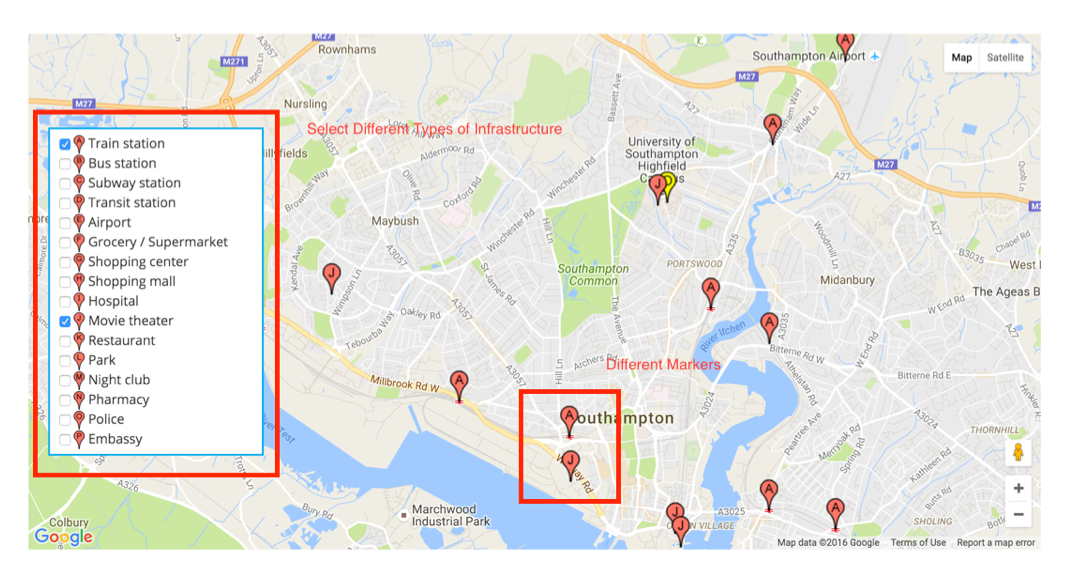
\includegraphics[width=15cm]{./img/Picture27}
  \caption{Infrastructure Part}
  \label{Figure:figex}
\end{figure}

\begin{figure}[H]
  \centering
  
\includegraphics[width=8cm]{./img/Picture28}
  \caption{Zero Results}
  \label{Figure:figex}
\end{figure}



\section{Summary}


This chapter focuses on the implementation of this system. At first, this chapter briefly introduces the technologies and tools used for implementing this system. Then, it explains how the main components of this system are implementation with several screenshots and part of codes provided.

%% ----------------------------------------------------------------
%% Test.tex
%% ---------------------------------------------------------------- 

\chapter{Testing and Evaluation} \label{Chapter:Testing and Evaluation}

This chapter will provide information about the testing and evaluation process of this system. First of all, functional testing will be carried out to identify whether this system meets the functional requirement specifications. Afterwards, non-functional testing will be conducted to check whether the system can achieve a high quality. At last, this chapter will introduce a comparative survey and analyse the survey results for system evaluation.



\section{System Testing}

System testing is a crucial phase in the software development lifecycle because it ensures the software system can conform to all user requirements and achieve a high quality. The system testing process is normally divided into functional testing and non-functional testing. This section will firstly introduce the functional testing and then non-functional testing of this system. 

\subsection{Functional Testing}
Functional testing is a process that checks software systems to ensure that they have all required functionalities that are specified within the functional requirements. In this project, functional testing verifies the functionalities of the system without peering into its internal structure. Therefore, the testing process only focuses on whether the actual outputs of this system match expectations, given certain input actions. Table 7.1 displays the test cases designed for functional testing with their descriptions, and Table 7.2 provides the result of each test case in the testing process.


\begin{table}[H]
\centering
\caption{Descriptions of Test Cases}
\label{my-label}
\begin{tabular}{|l|p{4cm}|p{8cm}|}
\hline
\textbf{ID} & \textbf{Test Scenario}                        & \textbf{Test Case}                                                               \\ \hline
TC-1        & Check search functionality                    & Check response on searching universities and courses                             \\ \hline
TC-2        & Check functionalities in ranking table part   & Check response on interacting with ranking table part                            \\ \hline
TC-3        & Check functionalities in course location part & Check response on interacting with the map in course location part               \\ \hline
TC-4        & Check functionalities in weather part         & Check response on interacting with the charts in weather part                    \\ \hline
TC-5        & Check functionalities in criminality part     & Check response on interacting with the map and the pie chart in criminality part \\ \hline
TC-6        & Check functionalities in infrastructure part  & Check response on interacting with the map in infrastructure part                \\ \hline
\end{tabular}
\end{table}



\begin{landscape}
\begin{center}
\begin{longtable}{|p{1cm}|p{3.5cm}|p{4cm}|p{3cm}|p{5cm}|p{2.5cm}|p{1cm}|}
\caption{Results of Functional Testing} \label{tab:long} \\

\hline \multicolumn{1}{|c|}{\textbf{ID}}   &  \multicolumn{1}{|c|}{\textbf{Pre-conditions}}  &  \multicolumn{1}{|c|}{\textbf{Test Steps}}  &  \multicolumn{1}{|c|}{\textbf{Test Data}} &  \multicolumn{1}{|c|}{\textbf{Expected Results}} &  \multicolumn{1}{|c|}{\textbf{Actual Results}} &  \multicolumn{1}{|c|}{\textbf{Pass/Fail}} \\ \hline 
\endfirsthead

\multicolumn{7}{c}%
{{\bfseries \tablename\ \thetable{} -- continued from previous page}} \\
\hline \multicolumn{1}{|c|}{\textbf{ID}}  &  \multicolumn{1}{|c|}{\textbf{Pre-conditions}}  &  \multicolumn{1}{|c|}{\textbf{Test Steps}}  &  \multicolumn{1}{|c|}{\textbf{Test Data}} &  \multicolumn{1}{|c|}{\textbf{Expected Results}} &  \multicolumn{1}{|c|}{\textbf{Actual Results}} &  \multicolumn{1}{|c|}{\textbf{Pass/Fail}} \\ \hline 
\endhead

%\hline \multicolumn{7}{|r|}{{Continued on next page}} \\ \hline
\endfoot

%\hline \hline
%\endlastfoot

TC-1 & The users enter this website’s homepage & 1.Enter a university and a course \newline 2.Select from suggestions
 & University of Southampton, Computer Science & The webpage displays information about University of Southampton and Computer Science & As Expected & Pass \\ \hline
TC-2 &  The webpage displays the ranking table part & 1.Enter a university  \newline
2.Click the buttons in the table & University of Southampton & The ranking table shows the ranking information about University of Southampton & As Expected & Pass \\ \hline
TC-3 & The webpage displays the map in course location part & / & / & The map shows the location of University of Southampton and the geographic proximity and driving time from it to several metropolis & As Expected & Pass \\ \hline
TC-4 & The webpage displays the charts in weather part & 1.Click the legends below the charts  \newline
2.Hover over the lines or charts & / & The charts show the lines or bars and the tooltips about the weather in Southampton according to the test steps  & As Expected & Pass \\ \hline
TC-5 & The webpage displays the map in criminality part & 1.Select different months  \newline
2.Hover over the circles  & May 2016 & The map and pie chart display information about criminality in Southampton in May 2016 and the tooltips of different location & As Expected & Pass \\ \hline
TC-6 & The webpage displays the map in infrastructure part & 1.Select airport  \newline 2.Select train station
 & Airport, Train station & The map displays the location of airports and train stations in Southampton & As Expected & Pass \\ \hline



\end{longtable}
\end{center}
\end{landscape}

\subsection{Non-functional Testing}

Non-functional testing, which consists of various testings, is used to test all non-functional attributes of software systems and ensures they can achieve a high quality. However, only several testings in non-functional testing are carried out in this project due to the time limit.   

\subsubsection{Compatibility Testing}

Compatibility testing, part of software non-functional tests, is testing conducted on the application to evaluate the application's compatibility with the different environment. Because this system is a web application, it should be compatible with different browsers. The compatibility testing of this system proved that it is compatible with commonly-used web browsers (Chrome, Firefox, IE and Safari).


\subsubsection{Usability Testing}

The user interface design follows the principles of modern user interaction and responsive web design. So, the results of the usability testing shows the user interface of this system is easy to understand and this system can be accessed via different devices (PC, smartphones and tablets).

\subsubsection{Accessibility Testing}

Several tools listed in Table 7.3 are used to test the accessibility of this system, which helps find errors that were difficult to discover such as wrong tag properties, or invalid links. The outcomes of accessibility testing prove that this system can meet Web accessibility standards provided by W3C.

%\begin{table}[H]
%\centering
%\caption{Tools Used for Accessibility Testing}
%\label{my-label}
%\begin{tabular}{|l|l|}
%\hline
%\textbf{Tool}                 & \textbf{Description}                       \\ \hline
%W3C Link Checker              & Check links and anchors in webpages \\ \hline
%W3C Markup Validation Service & Check the markup (HTML) of this web application \\ \hline
%W3C CSS Validation Service    & Check Cascading Style Sheets (CSS) \\ \hline
%JSLint                        & Checks errors and potential problems in JavaScript \\ \hline
%\end{tabular}
%\end{table}

\section{System Evaluation}

System evaluation is a process of assessing the performance of a software system to identify whether it could be applied in the real world. This section will introduce a survey that was used for system evaluation and then analyse the results of the survey and the feedbacks from respondents.


\subsection{Survey Design
}

In order to evaluate this system, the comparative survey methodology was used to design the survey. Specifically, the survey aimed to compare this system with UCAS, an official website for international students to search for universities and courses in the UK, and identify the advantages and disadvantage of this system. In this survey, the respondents were firstly asked to complete several tasks in a task list. The aim of the task list was to help them understand how to use this system and compare it with UCAS by completing a list of tasks. Afterwards, the respondents were asked to complete the questionnaire hosted in iSurvey. The questionnaire consisted of four questions using the Likert scale, ranging from strongly disagree to strongly agree, and several open-ended questions to allow students give some feedbacks and further improvements about this system according to their experience in completing the task list. The task list and questionnaire were both sent to the respondents via emails. The task list and questionnaire can be found in Appendix B and Appendix C respectively.


\subsection{Results Analysis}


There were 17 respondents who took part in this survey and they are international students who planned to study in the UK for their higher education. Figure 7.1 shows most (82.4\%) of the respondents have previous experience in using websites like UCAS to search universities and courses for their higher education. 


\begin{figure}[H]
  \centering
  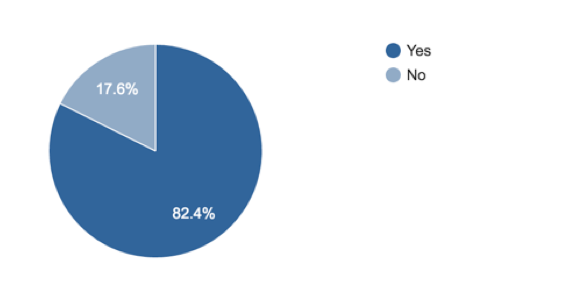
\includegraphics[width=10cm]{./img/Picture29}
  \caption{Previous Experience in Using Websites Like UCAS
}
  \label{Figure:figex}
\end{figure}


The following tables display the respondents’ opinions on this system from different aspects after completing the tasks in the task list. Table 7.3 shows most respondents agreed the user interface of this system were easy to learn and understand, and the user experience was good. However, some respondents thought some improvements should be considered in the user interface design and the user experience. Firstly, some of them complained that the loading time was a little bit long when they entered this system at the first time. Secondly, some respondents suggested that a back-to-top button could be added in the webpage to enable them to easily return to the search bar. Thirdly, some respondents pointed out that it was not convenient for them to compare several universities and cities at the same time and what they could do was searching and compare them over and over again. 


\begin{table}[H]
\centering
\caption{Opinions on the UI and UX
}
\label{my-label}
\begin{tabular}{|p{4cm}|c|c|c|c|c|c|c|}
\hline
                & \textbf{1} & \textbf{2} & \textbf{3} & \textbf{4} & \textbf{5} & \textbf{Weighted Mean} & \textbf{Interpretation} \\ \hline
User Interface  & 0          & 0          & 0          & 11         & 6          & 4.35                   & Agree                   \\ \hline
User Experience & 0          & 0          & 1          & 11         & 5          & 4.23                   & Agree                   \\ \hline
\end{tabular}
\end{table}


Table 7.4 shows the respondents’ opinions on the contents provided in this system. Most respondents strongly agreed that the contents provided in Course Location, Criminality and Infrastructure part were helpful for their destination choices.  The reason for this opinion was some of them thought course location, safety and infrastructure had great influences on their decision making for higher education, while others thought those contents could allow them to gain insights into universities from a different perspective. Some respondents thought the weather forecasts could give them a basic understanding of the weather in different cities, but it would more helpful if the historical information could be provided in this system. Moreover, some respondents hoped this system could provide some detailed descriptions about universities and courses in University\&Course part and some charts in Rankings Table part.

\begin{table}[H]
\centering
\caption{Opinions on Contents of This System}
\label{my-label}
\begin{tabular}{|p{4cm}|c|c|c|c|c|c|c|}
\hline
                   & \textbf{1} & \textbf{2} & \textbf{3} & \textbf{4} & \textbf{5} & \textbf{Weighted Mean} & \textbf{Interpretation} \\ \hline
University\&Course & 0          & 2          & 12         & 3          & 0          & 3.05                   & Neutral                 \\ \hline
Ranking Table      & 0          & 0          & 10         & 7          & 0          & 3.41                   & Neutral                 \\ \hline
Course Location    & 0          & 0          & 0          & 6          & 11         & 4.64                   & Strongly Agree          \\ \hline
Weather            & 0          & 1          & 4          & 7          & 5          & 3.94                   & Agree                   \\ \hline
Criminality        & 0          & 0          & 0          & 8          & 9          & 4.52                   & Strongly Agree          \\ \hline
Infrastructure     & 0          & 0          & 0          & 3          & 14         & 4.82                   & Strongly Agree          \\ \hline
\end{tabular}
\end{table}

Although this system has some shortcomings, most respondents agreed that this system was more helpful than UCAS (see Table 7.5), because they thought the information and visualisations provided in this system can provide comprehensive descriptions of universities and cities in the UK and help them make informed decisions. Besides, as shown in Figure 30, all of them were willing to recommend this system to their friends or peers if this system is applied in the real world. 

\begin{table}[H]
\centering
\caption{Comparison with UCAS
}
\label{my-label}
\begin{tabular}{|p{4cm}|c|c|c|c|c|c|c|}
\hline
                & \textbf{1} & \textbf{2} & \textbf{3} & \textbf{4} & \textbf{5} & \textbf{Weighted Mean} & \textbf{Interpretation} \\ \hline
More Helpful Than UCAS  & 0          & 0          & 1          & 10         & 6          & 4.29                   & Agree                   \\ \hline 
\end{tabular}
\end{table}


\begin{figure}[H]
  \centering
  
\includegraphics[width=11cm]{./img/Picture30}
  \caption{Willingness to Recommend This System
}
  \label{Figure:figex}
\end{figure}


\section{Summary}

This chapter introduces the testing and evaluation process of this system. The black box test is used to test the functionalities of this system, and the testing results proved that the functionalities of this system can work well and meet all user requirements. Besides, this system is evaluated using a comparative evaluation. Specially, a comparative survey containing a task list and an online questionnaire are used to compare this system with UCAS and gather the respondents’ opinions on this system. Though the results of evaluation show that this system has some shortcomings, the respondents thought this system helpful for international students’ destination choices in the UK.

%% ----------------------------------------------------------------
%% Conclusions.tex
%% ---------------------------------------------------------------- 
\chapter{Conclusion} \label{Chapter: Conclusion}
This chapter will firstly propose the future work that could improve this project based on the results of testing and evaluation. Afterwards, the critical reflection will reflect the learning outcomes and challenges by completing this project. Finally, the chapter will summarize this project based on the previous chapters.


\section{Future Work}

Due to the project constraints, the system can only offer functionalities that were initially identified and planned. Therefore, there are still some future work for this system. Firstly, a database can be added in this system to improve the stability and functionality. Although the usage of open data APIs can save time and obtain latest data, open APIs cannot be accessed without internet connection. The usage of a database allows to store the open datasets locally and ensures this system can be available at any time. Moreover, using a database make it possible to add more functionalities, such as login and registration. Secondly, open datasets about historical weather should be provided in this system, because some respondents suggested that information about historical weather is more helpful for them to compare the weather of different cities. Thirdly, the system should be improved to allow students to compare several universities and cities at the same time, which can improve the user experience. The usage of the database provides probabilities for this improvement. Lastly, more open datasets and data visualizations should be included in this system, especially in University\&Course and Ranking Table, and the web applications mentioned in section 2.3 are great examples.

\section{Critical Reflection}

It was a really challenge for me to go through the whole process of this project, because I have never completed a project independently before. Therefore, the completion of this project means the ending of a great journey of learning, which enriched my understanding on several areas and improved my practical skills. Firstly, background research on international students’ higher education destination choices, open data and data visualisation provided me with a great understanding of the relationship between them, which resulted in the final system of this project. Secondly, my project management understanding was improved throughout this project, because I had to choose a suitable software development methodology, make an appropriate plan and identify the potential risks to ensure this project can meet user requirements on time and within budget limits. Thirdly, the system design phase allows me to realise the importance of the stakeholders when developing a new idea, which make systems more than just a software tool. Fourthly, the implementation phase prompted me to learn some new technologies and tools to development a software system, though sometimes this phase was tough and dull. Lastly, I learned that the implementation phase is not the whole of the software development lifecycle, testing and evaluation are also crucial to the completion of a software system. 

Although I acquired a lot of knowledge and skill by experiencing each phase of this project, I also faced some challenges. As an international student, English is not my first language, so the first challenge for me was reading English literature and technical documentations. The second challenge was to search suitable open datasets and choose techniques and tools to implement this system. The third and biggest challenge was the implementation phase, because I did not learn JavaScript before and had to learn it from scratch and use it to develop this system within time limit.  However, the completion of this project means that I succeeded to complete those challenges.

To summarize, the aims and objectives of this project were successfully fulfilled, even though there is still some future work ahead of improving current functionalities and add more ones based on the results of comparative evaluation. By completion of the project, I have some ideas how to proceed a software project and have faith in becoming a software developer in future career.

\section{Conclusion}


International students’ decision-making process for higher education is complex and often involved in multiple factors. However, the factors influencing this process vary from different student populations and can be influenced by social and economic events. The dissertation summarised several key factors that influence international students’ destination choices from some literature and conducted a survey to identify those factors influencing the decision-making process of international students who choose the UK as their destination countries. Based on the results of the survey, this system was carefully analysed and designed to meet user requirements. Afterwards, a complete, fully-functional system was developed using open data and data visualization to help international students make informed decisions for their higher education destination choices.  Moreover, the testing and evaluation phase was followed to guarantee the high quality of the system and also to validate that all the intended functionalities are delivered. The results of the comparative evaluation showed some improvements should be considered in this system. For instance, it will be more helpful for international students if this system can provide information about historical weather instead of weather forecast. However, this system provides the ability to international students to compare different information about the key factors influencing their higher education destination choices. 

In conclusion, this system proved to be helpful for international students when they decide destination choices for their higher education in the UK. More importantly, this system provides a new way to apply open data and data visualization in higher education.

%\bibliographystyle{ecs}
%\bibliography{ECS}

\appendix
%% ----------------------------------------------------------------
%% AppendixA.tex
%% ---------------------------------------------------------------- 
\chapter{Questionnaire for Requirement Analysis} \label{Chapter:Appendix A}

% Converted from Microsoft Word to LaTeX
% by Chikrii Softlab Word2TeX converter (version 5.0)
% Copyright (C) 1999-2011 Chikrii Softlab. All rights reserved.
% http://www.chikrii.com
% mailto: support@chikrii.com

% Warning: You are using Chikrii Softlab Word2TeX in TRIAL mode!
% In TRIAL mode some restrictions will apply.
% For more information please visit http://www.chikrii.com
% YOU CAN USE THIS FILE WITH THE SOLE PURPOSE OF EVALUATING Word2TeX.





\begin{center}
\textbf{Factors influencing foreign students' higher education destination 
choices in the UK}
\end{center}

\begin{center}
\textbf{Section 1. Basic Information}
\end{center}

Question 1.1

What is your highest level of education qualification before studying in 
your university?

$\bigcirc $ High School Diploma

$\bigcirc $ College Diploma

$\bigcirc $ Bachelor`s Degree

$\bigcirc $ Master's Degree

$\bigcirc $ Other


Question 1.2

Which level do you study in your university?

$\bigcirc $ Bachelor's Degree

$\bigcirc $ Master's Degree

$\bigcirc $ Doctor's Degree

$\bigcirc $ Other


Question 1.3

Which region is your university located in?

$\bigcirc $ Greater London

$\bigcirc $ England (except Greater London)

$\bigcirc $ Wales

$\bigcirc $ Scotland

$\bigcirc $ North Ireland

$\bigcirc $ Other


Question 1.4

Please explain why you choose this region or state the advantages of this 
region compared with other regions.

\begin{center}


\textbf{Section 2. Factors influencing your destination choices in the UK}
\end{center}

Question 2.1

To what extent do the following factors play a role in your destination 
university? (1 $=$ No influence, 5 $=$ Strongly influenced)

\begin{table}[H]
\begin{center}
\begin{tabular}{|p{6cm}|p{1cm}|p{1cm}|p{1cm}|p{1cm}|p{1cm}|}
\hline
& 
1& 
2& 
3& 
4& 
5 \\
\hline
University Ranking& 
$\bigcirc $& 
$\bigcirc $& 
$\bigcirc $& 
$\bigcirc $& 
$\bigcirc $ \\
\hline
Cost (tuition fee, living cost, travel cost, etc.) & 
$\bigcirc $& 
$\bigcirc $& 
$\bigcirc $& 
$\bigcirc $& 
$\bigcirc $ \\
\hline
Environment (climate, city size, city location, crime rate of city, etc.) & 
$\bigcirc $& 
$\bigcirc $& 
$\bigcirc $& 
$\bigcirc $& 
$\bigcirc $ \\
\hline
Recommendations (Word of mouth) & 
$\bigcirc $& 
$\bigcirc $& 
$\bigcirc $& 
$\bigcirc $& 
$\bigcirc $ \\
\hline
Entry requirements & 
$\bigcirc $& 
$\bigcirc $& 
$\bigcirc $& 
$\bigcirc $& 
$\bigcirc $ \\
\hline
Employment rate & 
$\bigcirc $& 
$\bigcirc $& 
$\bigcirc $& 
$\bigcirc $& 
$\bigcirc $ \\
\hline
International Student Population & 
$\bigcirc $& 
$\bigcirc $& 
$\bigcirc $& 
$\bigcirc $& 
$\bigcirc $ \\
\hline
\end{tabular}
\label{tab1}
\end{center}
\end{table}

Question 2.2

Please explain any answers from above question that need further 
clarification

Question 2.3

In terms of university ranking, to what extent do the following rankings 
play a role in your destination university? (1 $=$ No influence, 5 $=$ 
Strongly influenced)

\begin{table}[H]
\begin{center}
\begin{tabular}{|p{6cm}|p{1cm}|p{1cm}|p{1cm}|p{1cm}|p{1cm}|}
\hline
& 
1& 
2& 
3& 
4& 
5 \\
\hline
Guardian University Ranking & 
$\bigcirc $& 
$\bigcirc $& 
$\bigcirc $& 
$\bigcirc $& 
$\bigcirc $ \\
\hline
Times Higher Education University Ranking & 
$\bigcirc $& 
$\bigcirc $& 
$\bigcirc $& 
$\bigcirc $& 
$\bigcirc $ \\
\hline
QS University Ranking & 
$\bigcirc $& 
$\bigcirc $& 
$\bigcirc $& 
$\bigcirc $& 
$\bigcirc $ \\
\hline
US News Global Universities Ranking & 
$\bigcirc $& 
$\bigcirc $& 
$\bigcirc $& 
$\bigcirc $& 
$\bigcirc $ \\
\hline
Research Excellence Framework (REF)                                       & 
$\bigcirc $& 
$\bigcirc $& 
$\bigcirc $& 
$\bigcirc $& 
$\bigcirc $ \\
\hline
The Complete University Guide Ranking (CUG)                                                                            & 
$\bigcirc $& 
$\bigcirc $& 
$\bigcirc $& 
$\bigcirc $& 
$\bigcirc $ \\
\hline
Academic Ranking of World Universities (Shanghai JiaoTong Ranking)                                                          & 
$\bigcirc $& 
$\bigcirc $& 
$\bigcirc $& 
$\bigcirc $& 
$\bigcirc $ \\
\hline
\end{tabular}
\label{tab1}
\end{center}
\end{table}

Question 2.4

Please explain any answers from above question that need further 
clarification

Question 2.5

In terms of cost issues, to what extent do the following costs play a role 
in your destination university? (1 $=$ No influence, 5 $=$ Strongly 
influenced)

\begin{table}[H]
\begin{center}
\begin{tabular}{|p{6cm}|p{1cm}|p{1cm}|p{1cm}|p{1cm}|p{1cm}|}
\hline
& 
1& 
2& 
3& 
4& 
5 \\
\hline
Tuition fee & 
$\bigcirc $& 
$\bigcirc $& 
$\bigcirc $& 
$\bigcirc $& 
$\bigcirc $ \\
\hline
Living cost & 
$\bigcirc $& 
$\bigcirc $& 
$\bigcirc $& 
$\bigcirc $& 
$\bigcirc $ \\
\hline
Travel cost & 
$\bigcirc $& 
$\bigcirc $& 
$\bigcirc $& 
$\bigcirc $& 
$\bigcirc $ \\
\hline
\end{tabular}
\label{tab1}
\end{center}
\end{table}



Question 2.6 

Please explain any answers from above question that need further 
clarification

Question 2.7 

In terms of the environment, to what extent do the following information 
play a role in your destination university? (1 $=$ No influence, 5 $=$ 
Strongly influenced) 


\begin{table}[H]
\begin{center}
\begin{tabular}{|p{6cm}|p{1cm}|p{1cm}|p{1cm}|p{1cm}|p{1cm}|}
\hline
& 
1& 
2& 
3& 
4& 
5 \\
\hline
Campus environment & 
$\bigcirc $& 
$\bigcirc $& 
$\bigcirc $& 
$\bigcirc $& 
$\bigcirc $ \\
\hline
Climate (weather) & 
$\bigcirc $& 
$\bigcirc $& 
$\bigcirc $& 
$\bigcirc $& 
$\bigcirc $ \\
\hline
Crime rate of city  & 
$\bigcirc $& 
$\bigcirc $& 
$\bigcirc $& 
$\bigcirc $& 
$\bigcirc $ \\
\hline
City size  & 
$\bigcirc $& 
$\bigcirc $& 
$\bigcirc $& 
$\bigcirc $& 
$\bigcirc $ \\
\hline
City location (geographic proximity to capital city or London)                  & 
$\bigcirc $& 
$\bigcirc $& 
$\bigcirc $& 
$\bigcirc $& 
$\bigcirc $ \\
\hline
City infrastructure (airport, railway station, etc.)                                                                             & 
$\bigcirc $& 
$\bigcirc $& 
$\bigcirc $& 
$\bigcirc $& 
$\bigcirc $ \\
\hline
\end{tabular}
\label{tab1}
\end{center}
\end{table}


Question 2.8 

Please explain any answers from above question that need further 
clarification

Question 2.9 

In terms of recommendations, to what extent do the recommendations from 
following people play a role in your destination university? (1 $=$ No 
influence, 5 $=$ Strongly influenced) 

\begin{table}[H]
\begin{center}
\begin{tabular}{|p{6cm}|p{1cm}|p{1cm}|p{1cm}|p{1cm}|p{1cm}|}
\hline
& 
1& 
2& 
3& 
4& 
5 \\
\hline
Parents/Relatives  & 
$\bigcirc $& 
$\bigcirc $& 
$\bigcirc $& 
$\bigcirc $& 
$\bigcirc $ \\
\hline
Friends  & 
$\bigcirc $& 
$\bigcirc $& 
$\bigcirc $& 
$\bigcirc $& 
$\bigcirc $ \\
\hline
Agents     & 
$\bigcirc $& 
$\bigcirc $& 
$\bigcirc $& 
$\bigcirc $& 
$\bigcirc $ \\
\hline
University official website & 
$\bigcirc $& 
$\bigcirc $& 
$\bigcirc $& 
$\bigcirc $& 
$\bigcirc $ \\
\hline

\end{tabular}
\label{tab1}
\end{center}
\end{table}



Question 2.10 

Please explain any answers from above question that need further 
clarification

Question 2.11 

What else do you want to share with me about factors that influence your 
destination university in the UK?

\begin{center}
\textbf{Thank you for taking this questionnaire.}
\end{center}





%% ----------------------------------------------------------------
%% AppendixB.tex
%% ---------------------------------------------------------------- 
\chapter{Task List for Comparative Evaluation} \label{Chapter:Appendix B}

% Converted from Microsoft Word to LaTeX
% by Chikrii Softlab Word2TeX converter (version 5.0)
% Copyright (C) 1999-2011 Chikrii Softlab. All rights reserved.
% http://www.chikrii.com
% mailto: support@chikrii.com

% Warning: You are using Chikrii Softlab Word2TeX in TRIAL mode!
% In TRIAL mode some restrictions will apply.
% For more information please visit http://www.chikrii.com
% YOU CAN USE THIS FILE WITH THE SOLE PURPOSE OF EVALUATING Word2TeX.


\begin{center}
\textbf{Task List}
\end{center}

Here is the websites for UCAS and UnivGuide respectively:

UCAS: \underline {https://www.ucas.com/}

UnivGuide:~\underline {http://univguide.netlify.com/{\#}/}

Please search for these five universities in UCAS and UnivGuide respectively 
according to~the tasks in the following~list. 

After completing this task list, please fill in an online questionnaire 
based on your experience.

Here is the website for the online questionnaire:

\underline {https://www.isurvey.soton.ac.uk/21173}

PS: The aim of the task list is to help you understand how to use UnivGuide 
and compare this system with UCAS. Therefore, it is not necessary to 
complete all of these tasks.

\begin{enumerate}
\item[\textbullet] University of Southampton, Computer Science
\item[\textbullet] University of Cambridge, Computer Science
\item[\textbullet] University of Manchester, Computer Science
\item[\textbullet] University of Nottingham, Computer Science
\item[\textbullet] University College London, Computer Science
\item Find the university that has the highest tuition fee
\item Find the university that has the highest living cost of university accommodation
\item Find the university that has the highest ranking
\item Find the university that has the highest completion rate
\item Find the university whose traveling time to London is less than 2 hour
\item Find information on the criminality around University of Southampton in January 2016.
\item Find the university that is close to the embassy.
\item Find the university that has 3 train stations near it.
\end{enumerate}



%% ----------------------------------------------------------------
%% AppendixC.tex
%% ---------------------------------------------------------------- 
\chapter{Questionnaire for Comparative Evaluation} \label{Chapter:Appendix C}

% Converted from Microsoft Word to LaTeX
% by Chikrii Softlab Word2TeX converter (version 5.0)
% Copyright (C) 1999-2011 Chikrii Softlab. All rights reserved.
% http://www.chikrii.com
% mailto: support@chikrii.com

% Warning: You are using Chikrii Softlab Word2TeX in TRIAL mode!
% In TRIAL mode some restrictions will apply.
% For more information please visit http://www.chikrii.com
% YOU CAN USE THIS FILE WITH THE SOLE PURPOSE OF EVALUATING Word2TeX.


\begin{center}
\textbf{Comparative Questionnaire for System Evaluation}
\end{center}

Question 1.1

Did you ever use any websites like UCAS or this one to search for 
universities or courses for your higher education? 

$\bigcirc $ Yes

$\bigcirc $ No

Question 1.2

Compared with UCAS, do you agree that the user interface of this website are 
easy to learn and understand? (1 $=$ Strongly disagree, 5 $=$ Strongly 
agree) 

$\bigcirc $ Strongly agree

$\bigcirc $ Agree

$\bigcirc $ Neutral

$\bigcirc $ Disagree

$\bigcirc $ Strongly disagree

Question 1.3

If you do not strongly agree, please describe any improvements in the 
interface and design should be considered. 

Question 1.4

Compared with UCAS, do you agree that the information of each part is 
helpful for your higher education destination choices? (1 $=$ Strongly 
disagree, 5 $=$ Strongly agree) 

\begin{table}[H]
\begin{center}
\begin{tabular}{|p{4cm}|p{1.5cm}|p{1.5cm}|p{1.5cm}|p{1.5cm}|p{1.5cm}|}
\hline
& 
1 & 
2 & 
3 & 
4 & 
5 \\
\hline
University {\&} Course& 
$\bigcirc $& 
$\bigcirc $& 
$\bigcirc $& 
$\bigcirc $& 
$\bigcirc $ \\
\hline
Ranking Table& 
$\bigcirc $& 
$\bigcirc $& 
$\bigcirc $& 
$\bigcirc $& 
$\bigcirc $ \\
\hline
Course Location& 
$\bigcirc $& 
$\bigcirc $& 
$\bigcirc $& 
$\bigcirc $& 
$\bigcirc $ \\
\hline
Weather & 
$\bigcirc $& 
$\bigcirc $& 
$\bigcirc $& 
$\bigcirc $& 
$\bigcirc $ \\
\hline
Criminality& 
$\bigcirc $& 
$\bigcirc $& 
$\bigcirc $& 
$\bigcirc $& 
$\bigcirc $ \\
\hline
Infrastructure& 
$\bigcirc $& 
$\bigcirc $& 
$\bigcirc $& 
$\bigcirc $& 
$\bigcirc $ \\
\hline
\end{tabular}
\label{tab1}
\end{center}
\end{table}

Question 1.5

If you do not totally agree, please describe any improvements in information 
of each part should be considered.

Question 1.6

Compared with UCAS, do you agree that the overall user experience of this 
website is good? (1 $=$ Strongly disagree, 5 $=$ Strongly agree) 

$\bigcirc $ 1

$\bigcirc $ 2

$\bigcirc $ 3

$\bigcirc $ 4

$\bigcirc $ 5

Question 1.7

If you do not strongly agree, please describe any improvements in the 
overall user experience should be considered.

Question 1.8

Compared with UCAS, do you think this website is more helpful for you to 
decide your higher education destination choices? (1 $=$ Strongly disagree, 
5 $=$ Strongly agree) 

$\bigcirc $ 1

$\bigcirc $ 2

$\bigcirc $ 3

$\bigcirc $ 4

$\bigcirc $ 5

Question 1.9

If you do not totally agree, please explain the answer from above question 
to give further clarification.

Question 1.10

Are you willing to recommend this website to your friends or peers? 

$\bigcirc $ Yes

$\bigcirc $ No

Question 1.11

What additional information on the universities or cities would you like 
included on this website?

\begin{center}
\textbf{Thank you for taking this questionnaire.}
\end{center}


\backmatter
\bibliographystyle{unsrt}
\bibliography{ECS}
\end{document}
%% ----------------------------------------------------------------